\documentclass[a4paper,14pt,oneside,openany]{memoir}

%%% Задаем поля, отступы и межстрочный интервал %%%

\usepackage[left=10mm, right=15mm, top=20mm, bottom=20mm]{geometry} 

\usepackage[english, russian]{babel}    
\usepackage{longtable,ltcaption}                    % Длинные таблицы
\usepackage{multirow,makecell}                      % Улучшенное форматирование таблиц
\usepackage{booktabs}                               % Еще один пакет для красивых таблиц
\usepackage{soulutf8}                               % Поддержка переносоустойчивых подчёркиваний и зачёркиваний
\usepackage{icomma}                                 % Запятая в десятичных дробях
\usepackage{hyphenat}                               % Для красивых переносов
\usepackage{textcomp}                               % Поддержка "сложных" печатных символов типа значков иены, копирайта и т.д.
\usepackage[version=4]{mhchem}                      % Красивые химические уравнения
\usepackage{amsmath} 

\usepackage[utf8]{inputenc}

\usepackage{amsthm}
\usepackage{amssymb}
\usepackage{enumerate}
\usepackage{stmaryrd}
\usepackage{cmll}
\usepackage{mathrsfs}
\usepackage{proof}
\usepackage{tikz}
\usepackage{multicol}
\usepackage{mathabx}
\usepackage{pdflscape}
\usepackage{listings}
\usepackage{xcolor}

%opening
\title{}
\author{}

\definecolor{codegreen}{rgb}{0,0.6,0}
\definecolor{codegray}{rgb}{0.5,0.5,0.5}
\definecolor{codepurple}{rgb}{0.58,0,0.82}

\lstdefinestyle{mystyle}{
	keywordstyle=\color{codepurple},
	numberstyle=\tiny\color{codegray},
	stringstyle=\color{codegreen},
	basicstyle=\ttfamily\footnotesize,
	breakatwhitespace=false,         
	breaklines=true,                 
	captionpos=b,                    
	keepspaces=true,                 
	numbers=left,                    
	numbersep=5pt,                  
	showspaces=false,                
	showstringspaces=false,
	showtabs=false,                  
	tabsize=2
}

\lstset{style=mystyle}


\begin{document}

\thispagestyle{empty}

\begin{center}
	
	Национальный исследовательский университет ИТМО\\
	Факультет информационных технологий и программирования\\
	Прикладная матеметика и информатика\\
	
	\vspace{20pt}
	
\end{center}

\vfill

\begin{center}
	\textbf {\fontsize{100}{120}\selectfont Методы оптимизации
	} \\  
	Отчет по лабораторной работе №2
	
\end{center}

\vfill

\begin{flushright}
	
	\hfill {
		Работу \\
		выполняли: \\
		Кольченко Антон М32371 \\ 
		Гайнанов Ильдар М32371 \\ 
		Муфтиев Руслан М32331\\ 
	}
	\vspace{20pt}
	
\end{flushright}

\vfill

\begin{center}
	Санкт-Петербург\\
	2023
\end{center}

\chapter*{Введение}
\textbf{Постановка задачи:}

\begin{enumerate}
\item Реализуйте стохастический градиентный спуск для решения линейной регрессии. Исследуйте сходимость с разным размером батча (1 - SGD, 2, .., n - 1 - Minibatch GD, n - GD из предыдущей работы). 
\item 
	Подберите функцию изменения шага (learning rate scheduling), чтобы улучшить
	сходимость, например экспоненциальную или ступенчатую.
	\item Исследуйте модификации градиентного спуска (Nesterov, Momentum, AdaGrad,
	RMSProp, Adam).
	\item Исследуйте сходимость алгоритмов. Сравнить различные методы по скорости
	сходимости, надежности, требуемым машинным ресурсам (объем оперативной
	памяти, количеству арифметических операций, времени выполнения)
	\item Постройте траекторию спуска различных алгоритмов из одной и той же исходной точки с одинаковой точностью. В отчете наложить эту траекторию на рисунок с линиями равного уровня заданной функции.
	\item Реализуйте полиномиальную регрессию. Постройте графики восстановленной
	регрессии для полиномов разной степени.
	\item Модифицируйте полиномиальную регрессию добавлением регуляризации в модель (L1, L2, Elastic регуляризации).
	\item Исследуйте влияние регуляризации на восстановление регрессии.
\end{enumerate}

\chapter{Теоретическая часть}
\section{Стохастический градиентный спуск}
\subsection{Стохастический градиентный спуск с постоянным шагом}

Принцип работы: 

Фактически, стохастический градиентный спуск отличается от привычного нам только тем, что вместо градиента по всем переменным мы берем значения переменных только по некоторым.

Вход: функция $f:\mathbb{R}^n \rightarrow \mathbb{R}$, стартовая точка $x = (x_1,x_2,...,x_n)$, точность $\varepsilon$, размер шага $\lambda$, переменные для дифференцирования $vars$.

Зададим функцию $g_{vars}: \mathbb{R}^n \rightarrow \mathbb{R}^n: \begin{cases}
	g_{vars}(x)_i = \frac{df}{dx_i}(x), i \in vars \\
	g_{vars}(x)_i = 0, i \not \in vars
\end{cases}$

Выход: найденная точка локального минимума

Алгоритм:
\begin{enumerate}
	\item $x^{[k+1]} = x^{[k]} - \lambda g_{vars}(x^{[k]})$.
	\item Повторять шаги, пока  $|f(x^{[k+1]}) - f(x^{[k]})| > \varepsilon$.
\end{enumerate}

\subsection {Стохастический градиентный спуск с функцией шага}

Принцип работы: 

Все аналогично, только у нас есть функция, которая будет давать нам размер шага на текущий момент.

Вход: функция $f:\mathbb{R}^n \rightarrow \mathbb{R}$, стартовая точка $x = (x_1,x_2,...,x_n)$, точность $\varepsilon$, размер шага $\lambda: \mathbb{N} \rightarrow \mathbb{R}$, переменные для дифференцирования $vars$.

Выход: найденная точка локального минимума

Алгоритм:
\begin{enumerate}
	\item $x^{[k+1]} = x^{[k]} - \lambda(n) \cdot g_{vars}(x^{[k]})$.
	\item Повторять шаги, пока  $|f(x^{[k+1]}) - f(x^{[k]})| > \varepsilon$.
\end{enumerate}

\newpage

\section{Функции шага}

Все дальнейшие функции шага будут $\mathbb{N} \rightarrow \mathbb{R}$.

\subsection{Константная функция шага}

Параметры: $c \in \mathbb{R}^+$

$$f(n) = c$$.

\subsection{Основанная на времени функция шага}

Параметры: $d \in \mathbb{R}$ - параметр затухания, $f_0$ - начальный шаг. 

$$f(0) = f_0$$
$$f(n + 1) = \dfrac{f(n)}{1 + dn}$$. 

\subsection{Основанная на шаге функция шага}

Параметры: $d \in \mathbb{R}$ - параметр затухания, $r \in \mathbb{N}$ - частота уменьшения шага, $f_0$ - начальный размер шага.
$$f(n) = f_0d^{\left \lfloor{\frac{1 + n}{r}}\right \rfloor}$$.

\subsection{Экспоненциальная функция шага}

Параметры: $d \in \mathbb{R}$ - параметр затухания, $f_0$ - начальный размер шага.
$$f(n) = f_0e^{-dn}$$.
\newpage

\section{Модификации градиентного спуска}
\subsection{Momentum}
Вход: функция $f:\mathbb{R}^n \rightarrow \mathbb{R}$, стартовая точка $x = (x_1,x_2,...,x_n)$, точность $\varepsilon$, размер шага $\lambda$, переменные для дифференцирования $vars$, параметр $m \in [0;\ 1]$.

Выход: найденная точка локального минимума

Алгоритм:
\begin{enumerate}
	\item $v ^{[k+1]} = v^{[k]} \cdot m - \lambda \cdot g_{vars}(x^{[k]})$ 
	\item $x^{[k+1]} = x^{[k]} + v^{[k + 1]}$.
	\item Повторять шаги, пока  $|f(x^{[k+1]}) - f(x^{[k]})| > \varepsilon$.
\end{enumerate}

\subsection{Nesterov}
Вход: функция $f:\mathbb{R}^n \rightarrow \mathbb{R}$, стартовая точка $x = (x_1,x_2,...,x_n)$, точность $\varepsilon$, размер шага $\lambda$, переменные для дифференцирования $vars$, параметр $m \in [0;\ 1]$.

Выход: найденная точка локального минимума

Алгоритм:
\begin{enumerate}
	\item $v ^{[k+1]} = v^{[k]} \cdot m + (1 - m) \cdot g_{vars}(x^{[k]} - \lambda \cdot m \cdot v^{[k]})$ 
	\item $\delta = - \lambda \cdot v ^{[k+1]}$
	\item $x^{[k+1]} = x^{[k]} + \delta$.
	\item Повторять шаг 1, пока  $|f(x^{[k+1]}) - f(x^{[k]})| > \varepsilon$.
\end{enumerate}

\subsection{AdaGrad}
Вход: функция $f:\mathbb{R}^n \rightarrow \mathbb{R}$, стартовая точка $x = (x_1,x_2,...,x_n)$, точность $\varepsilon$, размер шага $\lambda$, переменные для дифференцирования $vars$.

Выход: найденная точка локального минимума

Алгоритм:
\begin{enumerate}
	\item $g' = g_{vars}(x^{[k]})$
	\item $G^{[k + 1]} = G^{[k]} + \textlangle g', g' \textrangle$
	\item $\delta = \dfrac{-\lambda \cdot g'}{\sqrt{G + \epsilon}} $ [$\epsilon$ - очень малое число, вводится для того, чтобы избежать деления на ноль]
	\item $x^{[k+1]} = x^{[k]} + \delta$.
	\item Повторять шаг 1, пока  $|f(x^{[k+1]}) - f(x^{[k]})| > \varepsilon$.
\end{enumerate}

\subsection{RMSProp}
Вход: функция $f:\mathbb{R}^n \rightarrow \mathbb{R}$, стартовая точка $x = (x_1,x_2,...,x_n)$, точность $\varepsilon$, размер шага $\lambda$, переменные для дифференцирования $vars$, параметр $\beta \in [0;\ 1]$.

Выход: найденная точка локального минимума

Алгоритм:
\begin{enumerate}
	\item $g' = g_{vars}(x^{[k]})$
	\item $s^{[k + 1]} = \beta \cdot s^{[k]} + (1 - \beta) \cdot \textlangle g', g' \textrangle$
	\item $\delta = \dfrac{-\lambda \cdot g'}{\sqrt{s + \epsilon}} $ [$\epsilon$ - очень малое число, вводится для того, чтобы избежать деления на ноль]
	\item $x^{[k+1]} = x^{[k]} + \delta$.
	\item Повторять шаг 1, пока  $|f(x^{[k+1]}) - f(x^{[k]})| > \varepsilon$.
\end{enumerate}

\subsection{Adam}
Вход: функция $f:\mathbb{R}^n \rightarrow \mathbb{R}$, стартовая точка $x = (x_1,x_2,...,x_n)$, точность $\varepsilon$, размер шага $\lambda$, переменные для дифференцирования $vars$, параметры $\beta_1, \beta_2 \in [0;\ 1]$.

Выход: найденная точка локального минимума

Алгоритм:
\begin{enumerate}
	\item $g' = g_{vars}(x^{[k]})$
	\item $v^{[k + 1]} = \beta_1 \cdot v^{[k]} + (1 - \beta_1) \cdot g'$
	\item $s^{[k + 1]} = \beta_2 \cdot s^{[k]} + (1 - \beta_2) \cdot \textlangle g', g' \textrangle$
	\item $v'^{[k + 1]} = \dfrac{v^{[k + 1]}}{1 - \beta_1^k}$
	\item $s'^{[k + 1]} = \dfrac{s^{[k + 1]}}{1 - \beta_2^k}$
	\item $\delta = \dfrac{-\lambda \cdot v'^{[k + 1]}}{\sqrt{s'^{[k + 1]} + \epsilon}} $ [$\epsilon$ - очень малое число, вводится для того, чтобы избежать деления на ноль]
	\item $x^{[k+1]} = x^{[k]} + \delta$.
	\item Повторять шаг 1, пока  $|f(x^{[k+1]}) - f(x^{[k]})| > \varepsilon$.
\end{enumerate}
\newpage
\section{Полиномиальная регрессия}
\quad\quad Постановка задачи: \\
Дано множество точек $\{(x_i, y_i)\ |\ x_i, y_i \in \mathbb{R}\}$.
Мы хотим найти зависимость $y$ от $x$ и выразить ее как $\sum_{i=0}^{p} c_ix^i + \epsilon.$ \\
Как это сделать? \\
Заведем функцию Mean Square Error от коэффицентов: 
$$MSE(c_0, c_1, ..., c_p) = \dfrac{1}{n}\sum_{k = 0}^{n} (\sum_{j = 0}^{p}c_jx^j_k - y_k)^2 + reg(\alpha \sum_{j = 0}^{p}|c_j| + \dfrac{1 - \alpha}{2}c_i^2)$$ 

Играясь с параметрами этой функции, можно получить MSE для всех регуляризаций: $$\begin{cases}
	\text{Без регуляризации} & reg=0 \\
	\text{L1 регуляризация} & reg>0, \alpha=1 \\
	\text{L2 регуляризация} & reg>0, \alpha=1 \\
	\text{Elastic регуляризация} & reg>0, 0 < \alpha < 1 \\
\end{cases}$$

Теперь, когда мы выбрали регуляризацию, мы можем найти наши коэффициенты. Как? Мы просто запускаем любой градиентный спуск, где $f(x):=MSE(c_0, c_1, ..., c_p)$.

\chapter{Практическая часть}

Здесь и далее $\varepsilon = 10^{-9}$.
 
\section{Стандартный стохастический градиентный спуск}
\subsection{Реализация стохастического градиентного спуска}
\begin{lstlisting}[language=Python, caption=Стохастический градиентный спуск]
	import numpy as np
	import matplotlib.pyplot as plt
	from tabulate import tabulate
	import pandas as pd
	import math
	
	def rand_indexes(n, m):
	    return np.random.choice(n, m, replace=False)
	
	
	def gen_f(n, k):
	    m = np.random.rand(n, n) * 2
	    Q, _ = np.linalg.qr(m)
	    D = np.diag(np.array([k] + [1] * (n - 1)))
	
	    result = Q @ D @ np.linalg.inv(Q)
	
	    def f_impl(x):
	        return x.T @ result @ x
	
	    def f(x):
	        return np.apply_along_axis(f_impl, 0, x)
	
	    return f
	
	
	def batch_gradient(f, x, m):
	    n = len(x)
	    indexes = rand_indexes(n, m)
	    h = np.array([[0.0] * n for i in range(n)])
	    for i in indexes:
	        h[i][i] = 1e-6
	
	    l = f(x[:, np.newaxis] + h)
	    r = f(x[:, np.newaxis] - h)
	
	    return (l - r) / (2*(1e-6))
	
	
	def gradient_descent(f, x, lr, batch_size, lim=500, eps_mode=False):
	    n = len(x)
	    points = []
	    points.append(x)
	    if eps_mode:
	        while not abs(f(x) - f(x - lr * (g := batch_gradient(f, x, batch_size)))) < eps:
	            x = x - lr * g
	            points.append(x)
	
	            if len(points) > lim:
	                return np.array(points)
	    else:
	        for _ in range(lim):
	            x = x - lr * (g := batch_gradient(f, x, batch_size))
	            points.append(x)
	
	    return np.array(points)
	
\end{lstlisting}

\begin{lstlisting}[language=Python, caption=Пример использования стохастического градиентного спуска]
	n = 20
	k = 1
	lr = 0.05
	f = gen_f(n, k)
	x = np.array([-1.0] * n)
	
	points = gradient_descent(f, x, lr, 1, eps_mode=True)
	
	plt.plot(list(map(f, points)))
	plt.show()
\end{lstlisting}

\begin{figure}[ht]
	\centering
	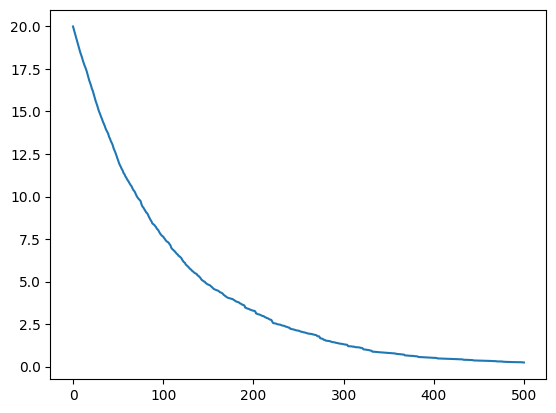
\includegraphics[width=0.5\textwidth]{img/1_1.png}
    \caption{График сходимости стохастического градиентного спуска}
\end{figure}

\newpage

\subsection{Сходимость стохастического градиентного спуска в зависимости от размера батча}

\begin{figure}[ht]
	\centering
	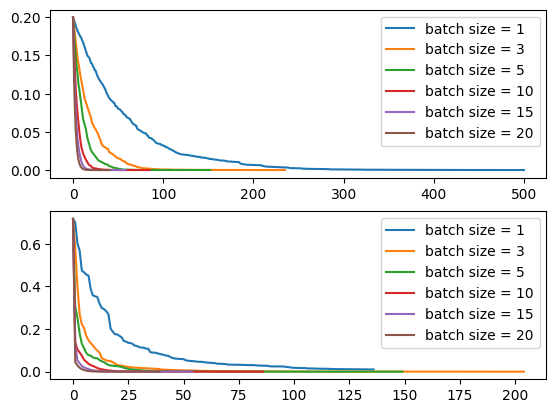
\includegraphics[width=0.5\textwidth]{img/1_2.png}
    \caption{Иллюстрация скорости сходимости градиентного спуска в зависимости от размера батча}
\end{figure}

\begin{table}[ht]
	\centering
	\resizebox{\textwidth}{!}{%
	\begin{tabular}{|c c c c c c c c c c c c c c c c c c c c|}
	\hline
	1&	2&	3&	4&	5&	6&	7&	8&	9&	10&	11&	12&	13&	14&	15&	16&	17&	18&	19&	20 \\
	\hline
	479.125&	500.7&	491.05&	401.1&	337.625&	290.75&	256.575&	230.175&	205.1&	186.15&	171.75&	158.8&	147.675&	137.85&	129.1&	120.875&	113.55&	108.1&	102.275&	96.85 \\
	\hline
	\end{tabular}}
    \caption{Таблица зависимости средней скорости сходимости функций в зависимости от размера батча}
\end{table}

Исследование скорости сходимости проводилось для 40 случайно сгенерированных функций, был взял средний результат среди всех запусков.

\subsection{Выводы}

\begin{itemize}
\item Наблюдается тенденция уменьшения количества шагов SGD с увеличением Batch Size. Стоит помнить, что хоть количество шагов и уменьшается, время исподнения программы может увеличиться из-за более дорогих вычислений градиента.
\end{itemize}

\newpage

\section{Функции изменения шага}



\begin{lstlisting}[language=Python, caption=Реализации функций изменения шага]
	def gen_const_lr(c):
	    return lambda: c
	
	
	def gen_timed_lr(lr0, d):
	    lr = [lr0]
	    n = [1]
	
	    def f():
	        result = lr[0]
	        lr[0] = lr[0] / (1 + d * n[0])
	        n[0] += 1
	        return result
	
	    return f
	
	
	def gen_stepped_lr(lr0, d, r):
	    n = [0]
	
	    def f():
	        n_ = n[0]
	        n[0] += 1
	        return lr0 * d ** (np.floor(1 + n_ / r))
	
	    return f
	
	
	def gen_exponential_lr(lr0, d):
	    n = [1]
	
	    def f():
	        n_ = n[0]
	        n[0] += 1
	        return lr0 * math.e ** (-d * n_)
	
	    return f
\end{lstlisting}

\begin{lstlisting}[language=Python, caption={Реализация функций стохастического градиентного спуска, использующих функции изменения шага}]
	def lrf_gradient_descent(f, x, lrf, batch_size, lim=1000, eps_mode=False):
	    n = len(x)
	    points = []
	    points.append(x)
	    lr = lrf()
	    if eps_mode:
	        while not abs(f(x) - f(x - lr * (g := batch_gradient(f, x, batch_size)))) < eps:
	            x = x - lr * g
	            points.append(x)
	            lr = lrf()
	
	            if len(points) > lim:
	                return np.array(points)
	    else:
	        for _ in range(lim):
	            x = x - lr * (g := batch_gradient(f, x, batch_size))
	            points.append(x)
	            lr = lrf()
	
	    return np.array(points)
	
	
	def lrf_gradient_descent_count(f, x, lrf, batch_size, lim=1000, eps_mode=False):
	    n = len(x)
	    points = 1
	    lr = lrf()
	    if eps_mode:
	        while not abs(f(x) - f(x - lr * (g := batch_gradient(f, x, batch_size)))) < eps:
	            x = x - lr * g
	            points += 1
	            lr = lrf()
	
	            if points > lim:
	                return points
	    else:
	        for _ in range(lim):
	            # while not abs(f(x) - f(x - lr * (g := batch_gradient(f,x, batch_size)))) < eps:
	            # print(f(x) - f(x - lr * (g := batch_gradient(f,x, batch_size))))
	            x = x - lr * (g := batch_gradient(f, x, batch_size))
	            points += 1
	            lr = lrf()
	
	    return points
\end{lstlisting}

Исследуем влияние функций изменения шага на сходимость функции стохастического спуска. Запустим на 10 случайно сгенерированных функциях, возьмем среднее арифметическое.

	\textbf{Block size 1} 
	
	Constant learning rate 
	
	\begin{tabular}{|c|c|c|c|c|c|c|}
	\hline 
	 &0.005 &0.010 &0.050 &0.100 &0.500 &1.000 \\
	 \hline 
	 &993.2 &774.9 &419.8 &249.6 &31.7 &773.9 \\
	 \hline 
	
	\end{tabular}
	
	Timed learning rate 
	
	\begin{tabular}{|c|c|c|c|c|c|}
	\hline 
	 &0.0001 &0.0005 &0.0010 &0.0050 &0.0100 \\
	 \hline 
	0.05 &458.1 &243.8 &181.3 &89.2 &65.1 \\
	 \hline 
	0.10 &392.0 &191.1 &152.9 &87.0 &65.6 \\
	 \hline 
	0.25 &110.7 &145.4 &134.1 &79.0 &60.4 \\
	 \hline 
	0.50 &36.7 &53.6 &99.1 &58.6 &54.0 \\
	 \hline 
	1.00 &139.6 &151.0 &131.1 &73.5 &58.2 \\
	 \hline 
	
	\end{tabular}
	
	Step-based learning rate (drops every 10 iterations) 
	
	\begin{tabular}{|c|c|c|c|c|c|c|}
	\hline 
	 &0.99 &0.95 &0.90 &0.75 &0.50 &0.33 \\
	 \hline 
	0.05 &535.6 &921.0 &880.1 &522.2 &232.0 &145.8 \\
	 \hline 
	0.10 &286.2 &492.6 &739.0 &466.5 &233.8 &149.8 \\
	 \hline 
	0.25 &107.8 &133.7 &262.5 &257.1 &227.7 &150.7 \\
	 \hline 
	0.50 &35.1 &39.4 &68.8 &256.2 &176.2 &137.3 \\
	 \hline 
	1.00 &352.7 &118.5 &69.2 &175.7 &139.9 &77.6 \\
	 \hline 
	2.00 &103.6 &433.2 &257.6 &277.3 &152.5 &131.4 \\
	 \hline 
	
	\end{tabular}
	
	Step-based learning rate (drops every 20 iterations) 
	
	\begin{tabular}{|c|c|c|c|c|c|c|}
	\hline 
	 &0.99 &0.95 &0.90 &0.75 &0.50 &0.33 \\
	 \hline 
	0.05 &633.7 &706.2 &903.4 &522.0 &228.4 &142.1 \\
	 \hline 
	0.10 &324.1 &661.8 &683.0 &471.8 &233.4 &148.6 \\
	 \hline 
	0.25 &104.8 &134.2 &342.0 &362.0 &222.2 &151.5 \\
	 \hline 
	0.50 &32.6 &35.6 &84.8 &216.0 &172.2 &141.1 \\
	 \hline 
	1.00 &366.4 &116.1 &76.4 &131.0 &105.5 &110.6 \\
	 \hline 
	2.00 &115.1 &357.4 &346.9 &269.7 &139.0 &126.2 \\
	 \hline 
	
	\end{tabular}
	
	Exponential learning rate 
	
	\begin{tabular}{|c|c|c|c|c|c|c|}
	\hline 
	 &0.99 &0.95 &0.90 &0.75 &0.50 &0.33 \\
	 \hline 
	0.05 &18.8 &19.2 &19.9 &23.5 &34.6 &52.5 \\
	 \hline 
	0.10 &19.2 &19.8 &21.0 &25.6 &36.3 &55.4 \\
	 \hline 
	0.25 &20.4 &20.1 &22.2 &26.6 &37.1 &55.6 \\
	 \hline 
	0.50 &20.4 &21.5 &22.8 &26.2 &38.5 &53.2 \\
	 \hline 
	1.00 &20.6 &21.7 &21.9 &23.1 &38.3 &49.0 \\
	 \hline 
	2.00 &21.2 &22.8 &22.9 &27.5 &39.0 &52.1 \\
	 \hline 
	
	\end{tabular}
	
	\textbf{Block size 3}
	
	Constant learning rate 
	
	\begin{tabular}{|c|c|c|c|c|c|c|}
	\hline 
	 &0.005 &0.010 &0.050 &0.100 &0.500 &1.000 \\
	 \hline 
	 &1001.0 &1001.0 &260.0 &138.0 &30.5 &466.9 \\
	 \hline 
	
	\end{tabular}
	
	Timed learning rate 
	
	\begin{tabular}{|c|c|c|c|c|c|}
	\hline 
	 &0.0001 &0.0005 &0.0010 &0.0050 &0.0100 \\
	 \hline 
	0.05 &421.9 &239.6 &179.4 &91.2 &67.8 \\
	 \hline 
	0.10 &201.9 &210.1 &161.5 &87.1 &66.0 \\
	 \hline 
	0.25 &55.8 &75.6 &97.7 &76.5 &59.3 \\
	 \hline 
	0.50 &30.0 &28.9 &28.8 &51.0 &52.4 \\
	 \hline 
	1.00 &121.4 &80.9 &70.4 &73.1 &56.6 \\
	 \hline 
	
	\end{tabular}
	
	Step-based learning rate (drops every 10 iterations) 
	
	\begin{tabular}{|c|c|c|c|c|c|c|}
	\hline 
	 &0.99 &0.95 &0.90 &0.75 &0.50 &0.33 \\
	 \hline 
	0.05 &298.8 &856.8 &930.7 &540.1 &255.8 &161.9 \\
	 \hline 
	0.10 &149.1 &214.3 &513.6 &463.3 &247.2 &166.7 \\
	 \hline 
	0.25 &55.5 &62.5 &81.9 &277.1 &217.0 &162.7 \\
	 \hline 
	0.50 &30.0 &29.5 &31.6 &58.9 &165.9 &145.4 \\
	 \hline 
	1.00 &317.8 &100.9 &62.0 &37.3 &82.7 &110.5 \\
	 \hline 
	2.00 &45.7 &53.2 &188.6 &138.5 &100.9 &106.8 \\
	 \hline 
	
	\end{tabular}
	
	Step-based learning rate (drops every 20 iterations) 
	
	\begin{tabular}{|c|c|c|c|c|c|c|}
	\hline 
	 &0.99 &0.95 &0.90 &0.75 &0.50 &0.33 \\
	 \hline 
	0.05 &301.7 &796.9 &938.8 &540.2 &258.9 &164.2 \\
	 \hline 
	0.10 &149.3 &223.1 &495.8 &453.2 &250.4 &165.9 \\
	 \hline 
	0.25 &52.3 &64.8 &81.3 &276.2 &209.1 &156.8 \\
	 \hline 
	0.50 &28.9 &28.2 &33.5 &65.9 &175.6 &137.0 \\
	 \hline 
	1.00 &313.7 &99.8 &63.4 &44.2 &99.3 &105.8 \\
	 \hline 
	2.00 &45.0 &55.3 &172.1 &108.3 &106.3 &110.6 \\
	 \hline 
	
	\end{tabular}
	
	Exponential learning rate 
	
	\begin{tabular}{|c|c|c|c|c|c|c|}
	\hline 
	 &0.99 &0.95 &0.90 &0.75 &0.50 &0.33 \\
	 \hline 
	0.05 &20.3 &20.9 &22.0 &26.9 &39.9 &59.0 \\
	 \hline 
	0.10 &21.0 &21.6 &23.0 &27.5 &39.7 &59.6 \\
	 \hline 
	0.25 &21.5 &22.7 &23.8 &28.4 &41.4 &59.8 \\
	 \hline 
	0.50 &22.1 &23.0 &24.5 &28.3 &40.7 &58.6 \\
	 \hline 
	1.00 &22.4 &22.8 &23.9 &28.5 &41.1 &54.8 \\
	 \hline 
	2.00 &22.9 &23.5 &23.9 &29.8 &42.9 &60.4 \\
	 \hline 
	
	\end{tabular}
	
	\textbf{Block size 5} 
	
	Constant learning rate 
	
	\begin{tabular}{|c|c|c|c|c|c|c|}
	\hline 
	 &0.005 &0.010 &0.050 &0.100 &0.500 &1.000 \\
	 \hline 
	 &1001.0 &796.9 &174.0 &87.9 &19.9 &321.6 \\
	 \hline 
	
	\end{tabular}
	
	Timed learning rate 
	
	\begin{tabular}{|c|c|c|c|c|c|}
	\hline 
	 &0.0001 &0.0005 &0.0010 &0.0050 &0.0100 \\
	 \hline 
	0.05 &299.8 &225.9 &174.1 &90.6 &67.6 \\
	 \hline 
	0.10 &101.4 &167.1 &148.5 &85.4 &64.8 \\
	 \hline 
	0.25 &34.5 &39.8 &39.9 &67.4 &55.8 \\
	 \hline 
	0.50 &20.6 &20.8 &18.8 &24.9 &38.3 \\
	 \hline 
	1.00 &115.4 &65.8 &55.6 &57.9 &53.5 \\
	 \hline 
	
	\end{tabular}
	
	Step-based learning rate (drops every 10 iterations) 
	
	\begin{tabular}{|c|c|c|c|c|c|c|}
	\hline 
	 &0.99 &0.95 &0.90 &0.75 &0.50 &0.33 \\
	 \hline 
	0.05 &187.6 &338.5 &804.7 &529.0 &261.9 &169.4 \\
	 \hline 
	0.10 &92.4 &116.3 &201.0 &426.5 &250.9 &167.6 \\
	 \hline 
	0.25 &36.2 &37.7 &45.8 &120.6 &206.2 &156.7 \\
	 \hline 
	0.50 &19.7 &18.3 &19.4 &27.9 &130.1 &132.6 \\
	 \hline 
	1.00 &275.2 &88.6 &52.5 &30.7 &29.2 &79.8 \\
	 \hline 
	2.00 &30.1 &34.1 &59.4 &76.4 &55.7 &70.5 \\
	 \hline 
	
	\end{tabular}
	
	Step-based learning rate (drops every 20 iterations) 
	
	\begin{tabular}{|c|c|c|c|c|c|c|}
	\hline 
	 &0.99 &0.95 &0.90 &0.75 &0.50 &0.33 \\
	 \hline 
	0.05 &190.4 &335.1 &803.1 &537.0 &259.8 &170.2 \\
	 \hline 
	0.10 &94.2 &119.5 &194.2 &425.0 &251.6 &168.8 \\
	 \hline 
	0.25 &36.2 &37.9 &45.8 &122.8 &201.7 &158.0 \\
	 \hline 
	0.50 &20.0 &20.7 &18.6 &27.9 &125.1 &129.3 \\
	 \hline 
	1.00 &307.5 &88.8 &52.9 &30.0 &26.3 &76.8 \\
	 \hline 
	2.00 &29.7 &32.4 &70.8 &85.5 &82.1 &71.9 \\
	 \hline 
	
	\end{tabular}
	
	Exponential learning rate 
	
	\begin{tabular}{|c|c|c|c|c|c|c|}
	\hline 
	 &0.99 &0.95 &0.90 &0.75 &0.50 &0.33 \\
	 \hline 
	0.05 &20.7 &21.7 &22.9 &27.3 &40.5 &60.6 \\
	 \hline 
	0.10 &21.5 &22.1 &23.7 &27.9 &41.5 &61.5 \\
	 \hline 
	0.25 &22.3 &22.9 &24.2 &28.4 &41.3 &60.9 \\
	 \hline 
	0.50 &22.5 &23.2 &24.2 &28.8 &39.8 &56.4 \\
	 \hline 
	1.00 &22.1 &22.8 &24.2 &27.5 &40.5 &54.0 \\
	 \hline 
	2.00 &23.1 &24.1 &25.0 &29.9 &40.7 &58.0 \\
	 \hline 
	
	\end{tabular}
	
	\textbf{Block size 7} 
	
	Constant learning rate 
	
	\begin{tabular}{|c|c|c|c|c|c|c|}
	\hline 
	 &0.005 &0.010 &0.050 &0.100 &0.500 &1.000 \\
	 \hline 
	 &1001.0 &592.5 &131.0 &65.2 &14.6 &233.1 \\
	 \hline 
	
	\end{tabular}
	
	Timed learning rate 
	
	\begin{tabular}{|c|c|c|c|c|c|}
	\hline 
	 &0.0001 &0.0005 &0.0010 &0.0050 &0.0100 \\
	 \hline 
	0.05 &183.3 &211.3 &168.3 &89.1 &66.7 \\
	 \hline 
	0.10 &69.3 &105.5 &125.5 &81.3 &63.4 \\
	 \hline 
	0.25 &24.6 &27.2 &28.8 &51.1 &49.1 \\
	 \hline 
	0.50 &14.5 &14.2 &13.9 &14.4 &18.8 \\
	 \hline 
	1.00 &115.4 &62.4 &57.8 &45.4 &44.7 \\
	 \hline 
	
	\end{tabular}
	
	Step-based learning rate (drops every 10 iterations) 
	
	\begin{tabular}{|c|c|c|c|c|c|c|}
	\hline 
	 &0.99 &0.95 &0.90 &0.75 &0.50 &0.33 \\
	 \hline 
	0.05 &139.7 &197.5 &527.0 &501.7 &259.2 &170.2 \\
	 \hline 
	0.10 &69.3 &79.9 &113.0 &368.4 &241.8 &168.1 \\
	 \hline 
	0.25 &26.0 &27.5 &31.5 &56.8 &181.6 &150.8 \\
	 \hline 
	0.50 &14.6 &14.6 &14.0 &17.7 &66.9 &116.2 \\
	 \hline 
	1.00 &150.4 &87.7 &49.0 &24.7 &17.2 &40.3 \\
	 \hline 
	2.00 &21.9 &24.7 &28.4 &73.8 &46.0 &55.4 \\
	 \hline 
	
	\end{tabular}
	
	Step-based learning rate (drops every 20 iterations) 
	
	\begin{tabular}{|c|c|c|c|c|c|c|}
	\hline 
	 &0.99 &0.95 &0.90 &0.75 &0.50 &0.33 \\
	 \hline 
	0.05 &138.8 &200.1 &524.2 &502.3 &257.5 &170.6 \\
	 \hline 
	0.10 &66.4 &81.4 &109.2 &359.2 &242.2 &168.1 \\
	 \hline 
	0.25 &26.3 &27.3 &31.5 &58.4 &179.3 &149.4 \\
	 \hline 
	0.50 &13.9 &13.5 &13.7 &16.8 &63.8 &117.9 \\
	 \hline 
	1.00 &123.5 &91.2 &50.1 &24.9 &16.7 &40.3 \\
	 \hline 
	2.00 &21.9 &23.9 &30.2 &71.7 &49.7 &51.8 \\
	 \hline 
	
	\end{tabular}
	
	Exponential learning rate 
	
	\begin{tabular}{|c|c|c|c|c|c|c|}
	\hline 
	 &0.99 &0.95 &0.90 &0.75 &0.50 &0.33 \\
	 \hline 
	0.05 &21.1 &21.9 &23.1 &28.0 &40.9 &60.7 \\
	 \hline 
	0.10 &21.7 &22.7 &23.8 &28.3 &41.8 &61.6 \\
	 \hline 
	0.25 &22.2 &23.1 &24.3 &28.8 &41.4 &58.6 \\
	 \hline 
	0.50 &22.5 &22.9 &24.1 &28.2 &39.6 &53.9 \\
	 \hline 
	1.00 &21.6 &22.6 &23.9 &27.2 &38.3 &52.9 \\
	 \hline 
	2.00 &22.8 &23.8 &25.0 &29.4 &42.3 &59.7 \\
	 \hline 
	
	\end{tabular}
	
	Block size 10 Constant learning rate 
	
	\begin{tabular}{|c|c|c|c|c|c|c|}
	\hline 
	 &0.005 &0.010 &0.050 &0.100 &0.500 &1.000 \\
	 \hline 
	 &843.3 &437.1 &92.3 &45.7 &36.2 &50.8 \\
	 \hline 
	
	\end{tabular}
	
	Timed learning rate 
	
	\begin{tabular}{|c|c|c|c|c|c|}
	\hline 
	 &0.0001 &0.0005 &0.0010 &0.0050 &0.0100 \\
	 \hline 
	0.05 &107.5 &177.5 &153.3 &86.0 &65.1 \\
	 \hline 
	0.10 &47.3 &56.1 &78.5 &75.0 &59.6 \\
	 \hline 
	0.25 &16.5 &16.6 &17.1 &22.4 &33.4 \\
	 \hline 
	0.50 &24.5 &19.5 &17.2 &12.4 &10.2 \\
	 \hline 
	1.00 &52.7 &44.6 &75.5 &32.8 &31.8 \\
	 \hline 
	
	\end{tabular}
	
	Step-based learning rate (drops every 10 iterations) 
	
	\begin{tabular}{|c|c|c|c|c|c|c|}
	\hline 
	 &0.99 &0.95 &0.90 &0.75 &0.50 &0.33 \\
	 \hline 
	0.05 &97.2 &125.2 &229.4 &459.0 &257.0 &170.0 \\
	 \hline 
	0.10 &47.3 &53.4 &65.9 &252.0 &230.0 &167.0 \\
	 \hline 
	0.25 &16.6 &17.6 &19.6 &29.7 &140.0 &137.0 \\
	 \hline 
	0.50 &25.3 &17.1 &13.3 &10.0 &21.6 &87.0 \\
	 \hline 
	1.00 &83.2 &56.1 &68.8 &28.9 &12.5 &11.0 \\
	 \hline 
	2.00 &17.1 &17.8 &18.9 &33.0 &27.2 &19.8 \\
	 \hline 
	
	\end{tabular}
	
	Step-based learning rate (drops every 20 iterations) 
	
	\begin{tabular}{|c|c|c|c|c|c|c|}
	\hline 
	 &0.99 &0.95 &0.90 &0.75 &0.50 &0.33 \\
	 \hline 
	0.05 &97.2 &125.2 &229.4 &459.0 &257.0 &170.0 \\
	 \hline 
	0.10 &47.3 &53.4 &65.9 &252.0 &230.0 &167.0 \\
	 \hline 
	0.25 &16.6 &17.6 &19.6 &29.7 &140.0 &137.0 \\
	 \hline 
	0.50 &25.3 &17.1 &13.3 &10.0 &21.6 &87.0 \\
	 \hline 
	1.00 &83.2 &56.1 &68.8 &28.9 &12.5 &11.0 \\
	 \hline 
	2.00 &17.1 &17.8 &18.9 &33.0 &27.2 &19.8 \\
	 \hline 
	
	\end{tabular}
	
	Exponential learning rate 
	
	\begin{tabular}{|c|c|c|c|c|c|c|}
	\hline 
	 &0.99 &0.95 &0.90 &0.75 &0.50 &0.33 \\
	 \hline 
	0.05 &21.4 &22.2 &23.5 &28.0 &41.5 &61.6 \\
	 \hline 
	0.10 &21.9 &22.9 &24.1 &28.6 &41.7 &61.3 \\
	 \hline 
	0.25 &22.2 &23.0 &24.4 &28.6 &40.6 &56.5 \\
	 \hline 
	0.50 &21.8 &22.6 &23.4 &27.0 &36.1 &44.6 \\
	 \hline 
	1.00 &20.2 &20.7 &21.8 &23.9 &30.9 &29.9 \\
	 \hline 
	2.00 &20.8 &21.5 &22.9 &26.4 &33.9 &43.0 \\
	 \hline 
	
	\end{tabular}
	
    \begin{table}[ht]\caption{Таблица зависимости средней скорости сходимости функций с разным размером батча в зависимости от выбора функции изменения шага.}
    \end{table}
    

    
    \subsection{Выводы}
    
    \begin{itemize}
    \item Очевидно, что лучше использовать нетривиальную функцию изменения шага. Что касается сравнения среди них, то они все достигают примерно одинаковых результатов. Но они в разной степени требовательны к подбору правилных параметров. Так, экспоненциальная функция в большинстве случаев все равно будет лучше константной. А с функцией, основанной на шаге, неправильные параметры с большей вероятностью приведут к результатам, которые значительно хуже.
    \end{itemize}
    
    \newpage
    
	\section {Модификации градиентного спуска}
	
	\begin{lstlisting}[language=Python, caption=Реализации различных модификаций стохастического градиентного спуска]
		def momentum_gd(f, x, lr, momentum, batch_size, lim=500, eps_mode=False):
		    n = len(x)
		    points = []
		    points.append(x)
		    v = np.array([0] * len(x))
		    if eps_mode:
		        while True:
		            v = momentum * v - lr * (g := batch_gradient(f, x, batch_size))
		
		            if abs(f(x) - f(x + v)) < eps:
		                break
		            x = x + v
		
		            points.append(x)
		
		            if len(points) > lim:
		                return np.array(points)
		    else:
		        for _ in range(lim):
		            v = momentum * v - lr * (g := batch_gradient(f, x, batch_size))
		            x = x + v
		            points.append(x)
		
		    return np.array(points)
		
		
		def nesterov_gd(f, x, lr, momentum, batch_size, lim=500, eps_mode=False):
		    n = len(x)
		    points = []
		    points.append(x)
		    v = np.array([0] * len(x))
		    if eps_mode:
		        while True:
		            v = momentum * v + (1 - momentum) * batch_gradient(f,
		                                                               x - lr * momentum * v, batch_size)
		            delta = - lr * v
		            if abs(f(x) - f(x + delta)) < eps:
		                break
		            x = x + delta
		
		            points.append(x)
		
		            if len(points) > lim:
		                return np.array(points)
		    else:
		        for _ in range(lim):
		            v = momentum * v + (1 - momentum) * batch_gradient(f,
		                                                               x - lr * momentum * v, batch_size)
		            delta = - lr * v
		            x = x + delta
		            points.append(x)
		
		    return np.array(points)
		
		
		def adagrad(f, x, lr, batch_size, lim=500, eps_mode=False):
		    ee = 1e-8
		    n = len(x)
		    points = []
		    points.append(x)
		    G = 0
		    if eps_mode:
		        while True:
		            g = batch_gradient(f, x, batch_size)
		            G += np.dot(g, g)
		            delta = - lr * g / np.sqrt(G + ee)
		            if abs(f(x) - f(x + delta)) < eps:
		                break
		            x = x + delta
		
		            points.append(x)
		
		            if len(points) > lim:
		                return np.array(points)
		    else:
		        for _ in range(lim):
		            g = batch_gradient(f, x, batch_size)
		            G += np.dot(g, g)
		            delta = - lr * g / np.sqrt(G + ee)
		            x = x + delta
		            points.append(x)
		
		    return np.array(points)
		
		
		def rmsprop(f, x, lr, beta, batch_size, lim=500, eps_mode=False):
		    ee = 1e-8
		    n = len(x)
		    points = []
		    points.append(x)
		    s = 0
		    if eps_mode:
		        while True:
		            g = batch_gradient(f, x, batch_size)
		            s = s * beta + (1 - beta) * np.dot(g, g)
		            delta = - lr * g / np.sqrt(s + ee)
		            if abs(f(x) - f(x + delta)) < eps:
		                break
		            x = x + delta
		
		            points.append(x)
		
		            if len(points) > lim:
		                return np.array(points)
		    else:
		        for _ in range(lim):
		            g = batch_gradient(f, x, batch_size)
		            s = s * beta + (1 - beta) * np.dot(g, g)
		            delta = - lr * g / np.sqrt(s + ee)
		            x = x + delta
		            points.append(x)
		
		    return np.array(points)
		
		
		def adam(f, x, lr, beta1, beta2, batch_size, lim=500, eps_mode=False):
		    ee = 1e-8
		    n = len(x)
		    points = []
		    points.append(x)
		    s = 0
		    v = np.array([0] * n)
		    if eps_mode:
		        while True:
		            g = batch_gradient(f, x, batch_size)
		            v = v * beta1 + (1 - beta1) * g
		            s = s * beta2 + (1 - beta2) * np.dot(g, g)
		            v_ = v / (1 - beta1 ** len(points))
		            s_ = s / (1 - beta2 ** len(points))
		            delta = - lr * v_ / np.sqrt(s_ + ee)
		            if abs(f(x) - f(x + delta)) < eps:
		                break
		            x = x + delta
		
		            points.append(x)
		
		            if len(points) > lim:
		                return np.array(points)
		    else:
		        for _ in range(lim):
		            g = batch_gradient(f, x, batch_size)
		            v = v * beta1 + (1 - beta1) * g
		            s = s * beta2 + (1 - beta2) * np.dot(g, g)
		            v_ = v / (1 - beta1 ** len(points))
		            s_ = s / (1 - beta2 ** len(points))
		            delta = - lr * v_ / np.sqrt(s_ + ee)
		            x = x + delta
		            points.append(x)
		
		    return np.array(points)
	\end{lstlisting}

	\begin{figure}[ht]
		\centering
		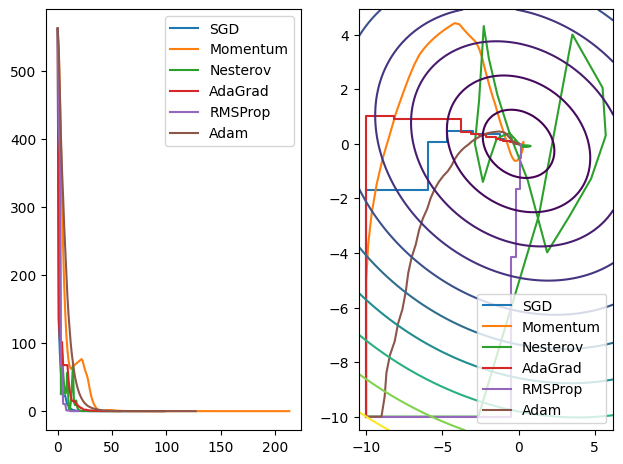
\includegraphics[width=0.65\textwidth]{img/3_1.png}
  \caption{Демонстрация графиков сходимости различных модификаций стохастического градиентного спуска при размере батча, равному 1}
  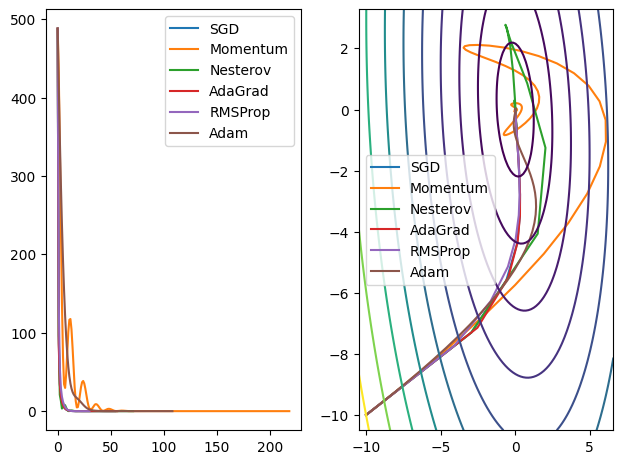
\includegraphics[width=0.65\textwidth]{img/3_2.png}
  	  \caption{Демонстрация графиков сходимости различных модификаций стохастического градиентного спуска при размере батча, равному 2}
	\end{figure}
	
	Рассмотрим влияние различных модификаций градиентного спуска на сходимость. Опять запустим на 10 случайно сгенерированных функциях, возьмем среднее арифметическое.
	
	\textbf{Block size 1}
	
	Standard SGD 
	
	\begin{tabular}{|c|c|c|c|c|c|c|c|}
	\hline 
	 &0.005 &0.010 &0.050 &0.100 &0.500 &1.000 &2.000 \\
	 \hline 
	 &501.0 &501.0 &487.8 &314.5 &35.2 &481.8 &85.3 \\
	 \hline 
	
	\end{tabular}
	
	Momentum SGD 
	
	\begin{tabular}{|c|c|c|c|c|c|c|c|}
	\hline 
	 &0.005 &0.010 &0.050 &0.100 &0.500 &1.000 &2.000 \\
	 \hline 
	0.1 &501.0 &501.0 &501.0 &403.2 &104.0 &479.1 &113.0 \\
	 \hline 
	0.2 &501.0 &501.0 &501.0 &371.2 &152.0 &382.4 &110.9 \\
	 \hline 
	0.3 &501.0 &501.0 &501.0 &325.6 &199.5 &311.4 &123.3 \\
	 \hline 
	0.4 &501.0 &501.0 &499.7 &294.0 &396.2 &255.4 &114.8 \\
	 \hline 
	0.5 &501.0 &501.0 &468.0 &243.3 &501.0 &237.2 &135.2 \\
	 \hline 
	0.6 &501.0 &501.0 &422.8 &182.1 &501.0 &230.2 &142.4 \\
	 \hline 
	0.7 &501.0 &501.0 &299.7 &166.3 &463.8 &241.0 &180.7 \\
	 \hline 
	0.8 &501.0 &501.0 &215.1 &215.3 &444.2 &255.5 &229.8 \\
	 \hline 
	0.9 &501.0 &478.1 &366.0 &501.0 &499.3 &445.0 &438.7 \\
	 \hline 
	
	\end{tabular}
	
	Nesterov SGD 
	
	\begin{tabular}{|c|c|c|c|c|c|c|c|}
	\hline 
	 &0.005 &0.010 &0.050 &0.100 &0.500 &1.000 &2.000 \\
	 \hline 
	0.1 &501.0 &501.0 &501.0 &439.3 &66.2 &501.0 &132.6 \\
	 \hline 
	0.2 &501.0 &501.0 &501.0 &454.7 &89.4 &501.0 &144.7 \\
	 \hline 
	0.3 &501.0 &501.0 &501.0 &475.6 &91.8 &501.0 &153.7 \\
	 \hline 
	0.4 &501.0 &501.0 &501.0 &480.2 &86.6 &501.0 &170.8 \\
	 \hline 
	0.5 &501.0 &501.0 &501.0 &483.8 &101.5 &501.0 &196.0 \\
	 \hline 
	0.6 &501.0 &501.0 &501.0 &486.9 &118.8 &498.4 &239.6 \\
	 \hline 
	0.7 &501.0 &501.0 &501.0 &487.1 &141.7 &490.5 &327.9 \\
	 \hline 
	0.8 &501.0 &501.0 &501.0 &490.7 &174.0 &478.3 &493.1 \\
	 \hline 
	0.9 &501.0 &501.0 &501.0 &466.3 &338.6 &501.0 &501.0 \\
	 \hline 
	
	\end{tabular}
	
	Adagrad 
	
	\begin{tabular}{|c|c|c|c|c|c|c|c|c|c|}
	\hline 
	 &0.005 &0.010 &0.050 &0.100 &0.500 &1.000 &2.000 &4.000 &8.000 \\
	 \hline 
	 &501.0 &501.0 &501.0 &501.0 &501.0 &501.0 &501.0 &458.0 &226.8 \\
	 \hline 
	
	\end{tabular}
	
	RMSProp 
	
	\begin{tabular}{|c|c|c|c|c|c|c|c|c|}
	\hline 
	 &0.005 &0.010 &0.050 &0.100 &0.500 &1.000 &2.000 &4.000 \\
	 \hline 
	0.900 &501.0 &501.0 &501.0 &501.0 &398.0 &457.4 &377.1 &501.0 \\
	 \hline 
	0.910 &501.0 &501.0 &501.0 &497.9 &492.9 &441.1 &501.0 &296.8 \\
	 \hline 
	0.920 &501.0 &501.0 &501.0 &501.0 &383.0 &418.3 &454.1 &454.6 \\
	 \hline 
	0.930 &501.0 &501.0 &501.0 &501.0 &404.0 &349.4 &411.6 &484.2 \\
	 \hline 
	0.940 &501.0 &501.0 &501.0 &501.0 &287.7 &378.4 &428.1 &501.0 \\
	 \hline 
	0.950 &501.0 &501.0 &501.0 &495.4 &280.0 &232.8 &370.7 &470.3 \\
	 \hline 
	0.960 &501.0 &501.0 &501.0 &501.0 &197.0 &193.4 &280.8 &377.8 \\
	 \hline 
	0.970 &501.0 &501.0 &501.0 &501.0 &216.7 &120.1 &132.4 &354.7 \\
	 \hline 
	0.980 &501.0 &501.0 &501.0 &488.4 &229.2 &123.5 &124.0 &202.9 \\
	 \hline 
	0.990 &501.0 &501.0 &501.0 &501.0 &244.7 &113.5 &73.3 &124.5 \\
	 \hline 
	0.999 &501.0 &501.0 &501.0 &482.3 &117.2 &75.2 &82.1 &100.8 \\
	 \hline 
	
	\end{tabular}
	
	Adam, lr = 0.1 
	
	\begin{tabular}{|c|c|c|c|c|c|c|c|c|c|}
	\hline 
	 &0.800 &0.825 &0.850 &0.875 &0.900 &0.925 &0.950 &0.975 &0.999 \\
	 \hline 
	0.800 &501.0 &501.0 &501.0 &501.0 &501.0 &501.0 &501.0 &501.0 &501.0 \\
	 \hline 
	0.825 &501.0 &501.0 &501.0 &501.0 &501.0 &501.0 &501.0 &501.0 &501.0 \\
	 \hline 
	0.850 &501.0 &501.0 &501.0 &501.0 &501.0 &501.0 &501.0 &501.0 &501.0 \\
	 \hline 
	0.875 &501.0 &501.0 &501.0 &501.0 &501.0 &501.0 &501.0 &501.0 &501.0 \\
	 \hline 
	0.900 &501.0 &501.0 &501.0 &501.0 &501.0 &501.0 &501.0 &501.0 &501.0 \\
	 \hline 
	0.925 &501.0 &501.0 &501.0 &501.0 &501.0 &501.0 &501.0 &501.0 &501.0 \\
	 \hline 
	0.950 &501.0 &501.0 &501.0 &501.0 &501.0 &501.0 &501.0 &501.0 &501.0 \\
	 \hline 
	0.975 &501.0 &501.0 &501.0 &501.0 &501.0 &501.0 &501.0 &501.0 &501.0 \\
	 \hline 
	0.999 &501.0 &501.0 &501.0 &501.0 &501.0 &501.0 &501.0 &501.0 &501.0 \\
	 \hline 
	
	\end{tabular}
	
	Adam, lr = 0.5 
	
	\begin{tabular}{|c|c|c|c|c|c|c|c|c|c|}
	\hline 
	 &0.800 &0.825 &0.850 &0.875 &0.900 &0.925 &0.950 &0.975 &0.999 \\
	 \hline 
	0.800 &501.0 &501.0 &501.0 &501.0 &501.0 &501.0 &501.0 &501.0 &501.0 \\
	 \hline 
	0.825 &501.0 &501.0 &501.0 &501.0 &501.0 &501.0 &501.0 &501.0 &501.0 \\
	 \hline 
	0.850 &501.0 &501.0 &501.0 &501.0 &501.0 &501.0 &501.0 &501.0 &501.0 \\
	 \hline 
	0.875 &501.0 &501.0 &501.0 &501.0 &501.0 &501.0 &501.0 &501.0 &501.0 \\
	 \hline 
	0.900 &501.0 &501.0 &501.0 &501.0 &501.0 &501.0 &501.0 &501.0 &501.0 \\
	 \hline 
	0.925 &501.0 &501.0 &501.0 &501.0 &501.0 &501.0 &501.0 &501.0 &501.0 \\
	 \hline 
	0.950 &501.0 &501.0 &501.0 &501.0 &501.0 &501.0 &501.0 &501.0 &501.0 \\
	 \hline 
	0.975 &444.7 &482.7 &480.5 &488.3 &501.0 &501.0 &501.0 &501.0 &501.0 \\
	 \hline 
	0.999 &483.7 &481.9 &490.2 &479.0 &481.0 &481.7 &491.7 &501.0 &501.0 \\
	 \hline 
	
	\end{tabular}
	
	Adam, lr = 1.0 
	
	\begin{tabular}{|c|c|c|c|c|c|c|c|c|c|}
	\hline 
	 &0.800 &0.825 &0.850 &0.875 &0.900 &0.925 &0.950 &0.975 &0.999 \\
	 \hline 
	0.800 &501.0 &501.0 &501.0 &501.0 &501.0 &501.0 &501.0 &501.0 &501.0 \\
	 \hline 
	0.825 &501.0 &501.0 &501.0 &501.0 &501.0 &501.0 &501.0 &501.0 &501.0 \\
	 \hline 
	0.850 &501.0 &501.0 &501.0 &501.0 &501.0 &501.0 &501.0 &501.0 &501.0 \\
	 \hline 
	0.875 &501.0 &501.0 &501.0 &501.0 &501.0 &501.0 &501.0 &501.0 &501.0 \\
	 \hline 
	0.900 &501.0 &501.0 &501.0 &501.0 &501.0 &501.0 &501.0 &501.0 &501.0 \\
	 \hline 
	0.925 &501.0 &501.0 &501.0 &501.0 &501.0 &501.0 &501.0 &501.0 &501.0 \\
	 \hline 
	0.950 &501.0 &501.0 &501.0 &501.0 &501.0 &501.0 &501.0 &501.0 &501.0 \\
	 \hline 
	0.975 &476.4 &475.4 &501.0 &501.0 &501.0 &501.0 &501.0 &501.0 &501.0 \\
	 \hline 
	0.999 &334.7 &314.1 &314.7 &320.1 &346.1 &394.3 &496.9 &501.0 &501.0 \\
	 \hline 
	
	\end{tabular}
	
	\textbf{Block size 3}
	
	Standard SGD 
	
	\begin{tabular}{|c|c|c|c|c|c|c|c|}
	\hline 
	 &0.005 &0.010 &0.050 &0.100 &0.500 &1.000 &2.000 \\
	 \hline 
	 &501.0 &501.0 &334.6 &168.6 &35.5 &322.5 &38.4 \\
	 \hline 
	
	\end{tabular}
	
	Momentum SGD 
	
	\begin{tabular}{|c|c|c|c|c|c|c|c|}
	\hline 
	 &0.005 &0.010 &0.050 &0.100 &0.500 &1.000 &2.000 \\
	 \hline 
	0.1 &501.0 &501.0 &322.3 &160.9 &44.3 &304.3 &56.8 \\
	 \hline 
	0.2 &501.0 &501.0 &289.3 &144.3 &59.9 &248.8 &68.2 \\
	 \hline 
	0.3 &501.0 &501.0 &251.6 &127.2 &79.3 &201.7 &69.4 \\
	 \hline 
	0.4 &501.0 &501.0 &213.8 &99.4 &120.8 &187.8 &82.0 \\
	 \hline 
	0.5 &501.0 &501.0 &178.7 &83.5 &240.3 &189.5 &99.0 \\
	 \hline 
	0.6 &501.0 &501.0 &134.4 &79.2 &478.5 &185.4 &131.7 \\
	 \hline 
	0.7 &501.0 &501.0 &103.7 &100.0 &493.0 &225.1 &156.3 \\
	 \hline 
	0.8 &501.0 &329.4 &138.8 &161.1 &437.6 &247.8 &234.7 \\
	 \hline 
	0.9 &281.1 &249.9 &301.8 &478.7 &496.1 &447.3 &416.7 \\
	 \hline 
	
	\end{tabular}
	
	Nesterov SGD 
	
	\begin{tabular}{|c|c|c|c|c|c|c|c|}
	\hline 
	 &0.005 &0.010 &0.050 &0.100 &0.500 &1.000 &2.000 \\
	 \hline 
	0.1 &501.0 &501.0 &348.0 &182.4 &37.3 &362.8 &62.2 \\
	 \hline 
	0.2 &501.0 &501.0 &359.6 &181.2 &40.0 &390.7 &73.9 \\
	 \hline 
	0.3 &501.0 &501.0 &357.8 &181.1 &38.7 &444.5 &81.7 \\
	 \hline 
	0.4 &501.0 &501.0 &362.2 &178.8 &42.4 &401.8 &97.4 \\
	 \hline 
	0.5 &501.0 &501.0 &365.8 &183.0 &47.6 &241.2 &124.4 \\
	 \hline 
	0.6 &501.0 &501.0 &370.6 &186.4 &62.5 &126.2 &159.2 \\
	 \hline 
	0.7 &501.0 &501.0 &355.4 &175.7 &80.6 &114.1 &254.3 \\
	 \hline 
	0.8 &501.0 &501.0 &352.2 &157.3 &116.9 &139.0 &501.0 \\
	 \hline 
	0.9 &501.0 &501.0 &283.8 &239.9 &216.1 &228.0 &360.2 \\
	 \hline 
	
	\end{tabular}
	
	Adagrad 
	
	\begin{tabular}{|c|c|c|c|c|c|c|c|c|c|}
	\hline 
	 &0.005 &0.010 &0.050 &0.100 &0.500 &1.000 &2.000 &4.000 &8.000 \\
	 \hline 
	 &501.0 &501.0 &501.0 &501.0 &501.0 &501.0 &501.0 &332.9 &114.1 \\
	 \hline 
	
	\end{tabular}
	
	RMSProp 
	
	\begin{tabular}{|c|c|c|c|c|c|c|c|c|}
	\hline 
	 &0.005 &0.010 &0.050 &0.100 &0.500 &1.000 &2.000 &4.000 \\
	 \hline 
	0.900 &501.0 &501.0 &501.0 &437.4 &421.0 &413.7 &455.9 &501.0 \\
	 \hline 
	0.910 &501.0 &501.0 &501.0 &418.7 &267.5 &284.3 &408.5 &501.0 \\
	 \hline 
	0.920 &501.0 &501.0 &501.0 &418.5 &121.3 &204.8 &363.5 &501.0 \\
	 \hline 
	0.930 &501.0 &501.0 &501.0 &426.0 &127.5 &123.9 &185.4 &453.5 \\
	 \hline 
	0.940 &501.0 &501.0 &501.0 &437.0 &133.9 &83.2 &182.6 &501.0 \\
	 \hline 
	0.950 &501.0 &501.0 &501.0 &446.4 &141.9 &85.4 &48.1 &314.1 \\
	 \hline 
	0.960 &501.0 &501.0 &501.0 &459.6 &151.4 &88.6 &48.8 &454.4 \\
	 \hline 
	0.970 &501.0 &501.0 &501.0 &475.3 &161.1 &89.5 &45.7 &316.3 \\
	 \hline 
	0.980 &501.0 &501.0 &501.0 &491.6 &172.7 &88.3 &43.7 &181.9 \\
	 \hline 
	0.990 &501.0 &501.0 &501.0 &501.0 &160.2 &67.7 &38.9 &42.2 \\
	 \hline 
	0.999 &501.0 &501.0 &501.0 &421.5 &46.1 &37.9 &42.3 &42.4 \\
	 \hline 
	
	\end{tabular}
	
	Adam, lr = 0.1 
	
	\begin{tabular}{|c|c|c|c|c|c|c|c|c|c|}
	\hline 
	 &0.800 &0.825 &0.850 &0.875 &0.900 &0.925 &0.950 &0.975 &0.999 \\
	 \hline 
	0.800 &501.0 &501.0 &501.0 &501.0 &501.0 &501.0 &501.0 &501.0 &501.0 \\
	 \hline 
	0.825 &501.0 &501.0 &501.0 &501.0 &501.0 &501.0 &501.0 &501.0 &501.0 \\
	 \hline 
	0.850 &501.0 &501.0 &501.0 &501.0 &501.0 &501.0 &501.0 &501.0 &501.0 \\
	 \hline 
	0.875 &501.0 &501.0 &501.0 &501.0 &501.0 &501.0 &501.0 &501.0 &501.0 \\
	 \hline 
	0.900 &501.0 &501.0 &501.0 &501.0 &501.0 &501.0 &501.0 &501.0 &501.0 \\
	 \hline 
	0.925 &501.0 &492.1 &501.0 &501.0 &501.0 &501.0 &501.0 &501.0 &501.0 \\
	 \hline 
	0.950 &473.7 &485.1 &501.0 &501.0 &501.0 &501.0 &501.0 &501.0 &501.0 \\
	 \hline 
	0.975 &494.2 &492.6 &493.9 &493.1 &496.0 &496.6 &501.0 &501.0 &501.0 \\
	 \hline 
	0.999 &501.0 &501.0 &501.0 &501.0 &501.0 &501.0 &501.0 &501.0 &501.0 \\
	 \hline 
	
	\end{tabular}
	
	Adam, lr = 0.5 
	
	\begin{tabular}{|c|c|c|c|c|c|c|c|c|c|}
	\hline 
	 &0.800 &0.825 &0.850 &0.875 &0.900 &0.925 &0.950 &0.975 &0.999 \\
	 \hline 
	0.800 &501.0 &501.0 &501.0 &501.0 &501.0 &501.0 &501.0 &501.0 &501.0 \\
	 \hline 
	0.825 &501.0 &501.0 &501.0 &501.0 &501.0 &501.0 &501.0 &501.0 &501.0 \\
	 \hline 
	0.850 &501.0 &501.0 &501.0 &501.0 &501.0 &501.0 &501.0 &501.0 &501.0 \\
	 \hline 
	0.875 &501.0 &501.0 &501.0 &501.0 &501.0 &501.0 &501.0 &501.0 &501.0 \\
	 \hline 
	0.900 &501.0 &501.0 &501.0 &501.0 &501.0 &501.0 &501.0 &501.0 &501.0 \\
	 \hline 
	0.925 &501.0 &501.0 &501.0 &501.0 &501.0 &501.0 &501.0 &501.0 &501.0 \\
	 \hline 
	0.950 &473.5 &501.0 &472.0 &501.0 &501.0 &501.0 &501.0 &501.0 &501.0 \\
	 \hline 
	0.975 &215.0 &226.6 &233.7 &254.7 &321.7 &485.2 &501.0 &501.0 &501.0 \\
	 \hline 
	0.999 &353.7 &340.8 &331.9 &323.8 &331.5 &345.7 &456.7 &501.0 &501.0 \\
	 \hline 
	
	\end{tabular}
	
	Adam, lr = 1.0 
	
	\begin{tabular}{|c|c|c|c|c|c|c|c|c|c|}
	\hline 
	 &0.800 &0.825 &0.850 &0.875 &0.900 &0.925 &0.950 &0.975 &0.999 \\
	 \hline 
	0.800 &501.0 &501.0 &501.0 &501.0 &501.0 &501.0 &501.0 &501.0 &501.0 \\
	 \hline 
	0.825 &501.0 &501.0 &501.0 &501.0 &501.0 &501.0 &501.0 &501.0 &501.0 \\
	 \hline 
	0.850 &501.0 &501.0 &501.0 &501.0 &501.0 &501.0 &501.0 &501.0 &501.0 \\
	 \hline 
	0.875 &501.0 &501.0 &501.0 &501.0 &501.0 &501.0 &501.0 &501.0 &501.0 \\
	 \hline 
	0.900 &501.0 &501.0 &501.0 &501.0 &501.0 &501.0 &501.0 &501.0 &501.0 \\
	 \hline 
	0.925 &501.0 &501.0 &501.0 &501.0 &501.0 &501.0 &501.0 &501.0 &501.0 \\
	 \hline 
	0.950 &501.0 &501.0 &501.0 &501.0 &501.0 &501.0 &501.0 &501.0 &501.0 \\
	 \hline 
	0.975 &155.9 &166.0 &188.4 &311.4 &501.0 &501.0 &501.0 &501.0 &501.0 \\
	 \hline 
	0.999 &175.0 &182.3 &181.2 &219.2 &238.1 &316.2 &446.5 &501.0 &501.0 \\
	 \hline 
	
	\end{tabular}
	
	\textbf{Block size 5}
	
	Standard SGD 
	
	\begin{tabular}{|c|c|c|c|c|c|c|c|}
	\hline 
	 &0.005 &0.010 &0.050 &0.100 &0.500 &1.000 &2.000 \\
	 \hline 
	 &501.0 &501.0 &217.2 &109.2 &23.5 &248.1 &26.3 \\
	 \hline 
	
	\end{tabular}
	
	Momentum SGD 
	
	\begin{tabular}{|c|c|c|c|c|c|c|c|}
	\hline 
	 &0.005 &0.010 &0.050 &0.100 &0.500 &1.000 &2.000 \\
	 \hline 
	0.1 &501.0 &501.0 &199.1 &102.2 &27.1 &261.9 &47.9 \\
	 \hline 
	0.2 &501.0 &501.0 &176.1 &89.1 &35.7 &277.2 &54.6 \\
	 \hline 
	0.3 &501.0 &501.0 &155.4 &78.3 &50.0 &273.2 &66.8 \\
	 \hline 
	0.4 &501.0 &501.0 &127.2 &60.2 &63.8 &253.9 &81.0 \\
	 \hline 
	0.5 &501.0 &501.0 &104.0 &56.0 &98.6 &214.2 &92.0 \\
	 \hline 
	0.6 &501.0 &426.4 &75.5 &60.2 &207.8 &213.5 &107.3 \\
	 \hline 
	0.7 &501.0 &316.7 &83.8 &87.4 &460.5 &223.3 &145.4 \\
	 \hline 
	0.8 &403.6 &175.7 &121.7 &139.9 &500.4 &284.6 &215.3 \\
	 \hline 
	0.9 &236.6 &229.2 &270.9 &362.4 &501.0 &438.7 &395.9 \\
	 \hline 
	
	\end{tabular}
	
	Nesterov SGD 
	
	\begin{tabular}{|c|c|c|c|c|c|c|c|}
	\hline 
	 &0.005 &0.010 &0.050 &0.100 &0.500 &1.000 &2.000 \\
	 \hline 
	0.1 &501.0 &501.0 &223.4 &113.4 &22.3 &286.6 &44.3 \\
	 \hline 
	0.2 &501.0 &501.0 &223.6 &113.0 &22.9 &315.3 &58.0 \\
	 \hline 
	0.3 &501.0 &501.0 &223.1 &112.8 &26.1 &313.7 &64.5 \\
	 \hline 
	0.4 &501.0 &501.0 &225.2 &111.2 &30.8 &309.5 &81.0 \\
	 \hline 
	0.5 &501.0 &501.0 &223.0 &112.3 &35.1 &91.1 &114.0 \\
	 \hline 
	0.6 &501.0 &501.0 &220.4 &103.5 &46.6 &52.4 &144.2 \\
	 \hline 
	0.7 &501.0 &501.0 &212.5 &96.9 &58.6 &56.8 &318.7 \\
	 \hline 
	0.8 &501.0 &501.0 &189.2 &112.8 &82.0 &72.4 &143.8 \\
	 \hline 
	0.9 &501.0 &501.0 &231.4 &211.9 &176.6 &141.8 &114.8 \\
	 \hline 
	
	\end{tabular}
	
	Adagrad 
	
	\begin{tabular}{|c|c|c|c|c|c|c|c|c|c|}
	\hline 
	 &0.005 &0.010 &0.050 &0.100 &0.500 &1.000 &2.000 &4.000 &8.000 \\
	 \hline 
	 &501.0 &501.0 &501.0 &501.0 &501.0 &501.0 &478.1 &230.3 &77.8 \\
	 \hline 
	
	\end{tabular}
	
	RMSProp 
	
	\begin{tabular}{|c|c|c|c|c|c|c|c|c|}
	\hline 
	 &0.005 &0.010 &0.050 &0.100 &0.500 &1.000 &2.000 &4.000 \\
	 \hline 
	0.900 &501.0 &501.0 &494.7 &324.8 &95.5 &60.6 &84.6 &263.6 \\
	 \hline 
	0.910 &501.0 &501.0 &496.0 &332.4 &99.1 &62.2 &85.8 &405.9 \\
	 \hline 
	0.920 &501.0 &501.0 &496.5 &338.6 &102.9 &65.3 &39.7 &311.0 \\
	 \hline 
	0.930 &501.0 &501.0 &499.2 &346.9 &108.4 &66.9 &39.5 &168.4 \\
	 \hline 
	0.940 &501.0 &501.0 &499.2 &356.5 &114.4 &68.8 &39.2 &264.1 \\
	 \hline 
	0.950 &501.0 &501.0 &501.0 &373.9 &119.6 &70.5 &39.6 &218.0 \\
	 \hline 
	0.960 &501.0 &501.0 &501.0 &393.3 &127.2 &71.8 &37.4 &122.6 \\
	 \hline 
	0.970 &501.0 &501.0 &501.0 &422.8 &134.9 &72.0 &34.6 &76.2 \\
	 \hline 
	0.980 &501.0 &501.0 &501.0 &462.1 &136.0 &66.1 &30.4 &31.4 \\
	 \hline 
	0.990 &501.0 &501.0 &501.0 &489.1 &119.8 &51.0 &26.3 &27.8 \\
	 \hline 
	0.999 &501.0 &501.0 &499.2 &308.9 &29.5 &24.9 &27.8 &27.3 \\
	 \hline 
	
	\end{tabular}
	
	Adam, lr = 0.1 
	
	\begin{tabular}{|c|c|c|c|c|c|c|c|c|c|}
	\hline 
	 &0.800 &0.825 &0.850 &0.875 &0.900 &0.925 &0.950 &0.975 &0.999 \\
	 \hline 
	0.800 &501.0 &501.0 &501.0 &501.0 &501.0 &501.0 &501.0 &501.0 &501.0 \\
	 \hline 
	0.825 &501.0 &501.0 &501.0 &501.0 &501.0 &501.0 &501.0 &501.0 &501.0 \\
	 \hline 
	0.850 &501.0 &501.0 &501.0 &501.0 &501.0 &501.0 &501.0 &501.0 &501.0 \\
	 \hline 
	0.875 &501.0 &501.0 &501.0 &501.0 &501.0 &501.0 &501.0 &501.0 &501.0 \\
	 \hline 
	0.900 &501.0 &501.0 &501.0 &501.0 &501.0 &501.0 &501.0 &501.0 &501.0 \\
	 \hline 
	0.925 &432.2 &501.0 &501.0 &501.0 &501.0 &501.0 &501.0 &501.0 &501.0 \\
	 \hline 
	0.950 &396.2 &408.3 &415.6 &452.6 &501.0 &501.0 &501.0 &501.0 &501.0 \\
	 \hline 
	0.975 &461.8 &465.6 &463.7 &470.3 &479.8 &494.0 &501.0 &501.0 &501.0 \\
	 \hline 
	0.999 &501.0 &501.0 &501.0 &501.0 &501.0 &501.0 &501.0 &501.0 &501.0 \\
	 \hline 
	
	\end{tabular}
	
	Adam, lr = 0.5 
	
	\begin{tabular}{|c|c|c|c|c|c|c|c|c|c|}
	\hline 
	 &0.800 &0.825 &0.850 &0.875 &0.900 &0.925 &0.950 &0.975 &0.999 \\
	 \hline 
	0.800 &501.0 &501.0 &501.0 &501.0 &501.0 &501.0 &501.0 &501.0 &501.0 \\
	 \hline 
	0.825 &501.0 &501.0 &501.0 &501.0 &501.0 &501.0 &501.0 &501.0 &501.0 \\
	 \hline 
	0.850 &501.0 &501.0 &501.0 &501.0 &501.0 &501.0 &501.0 &501.0 &501.0 \\
	 \hline 
	0.875 &501.0 &501.0 &501.0 &501.0 &501.0 &501.0 &501.0 &501.0 &501.0 \\
	 \hline 
	0.900 &501.0 &501.0 &501.0 &501.0 &501.0 &501.0 &501.0 &501.0 &501.0 \\
	 \hline 
	0.925 &466.6 &465.8 &501.0 &501.0 &501.0 &501.0 &501.0 &501.0 &501.0 \\
	 \hline 
	0.950 &173.5 &188.4 &356.1 &501.0 &501.0 &501.0 &501.0 &501.0 &501.0 \\
	 \hline 
	0.975 &183.8 &185.0 &196.0 &215.6 &250.6 &441.8 &501.0 &501.0 &501.0 \\
	 \hline 
	0.999 &259.2 &256.5 &246.2 &246.5 &266.7 &311.2 &431.0 &501.0 &501.0 \\
	 \hline 
	
	\end{tabular}
	
	Adam, lr = 1.0 
	
	\begin{tabular}{|c|c|c|c|c|c|c|c|c|c|}
	\hline 
	 &0.800 &0.825 &0.850 &0.875 &0.900 &0.925 &0.950 &0.975 &0.999 \\
	 \hline 
	0.800 &501.0 &501.0 &501.0 &501.0 &501.0 &501.0 &501.0 &501.0 &501.0 \\
	 \hline 
	0.825 &501.0 &501.0 &501.0 &501.0 &501.0 &501.0 &501.0 &501.0 &501.0 \\
	 \hline 
	0.850 &501.0 &501.0 &501.0 &501.0 &501.0 &501.0 &501.0 &501.0 &501.0 \\
	 \hline 
	0.875 &501.0 &501.0 &501.0 &501.0 &501.0 &501.0 &501.0 &501.0 &501.0 \\
	 \hline 
	0.900 &501.0 &501.0 &501.0 &501.0 &501.0 &501.0 &501.0 &501.0 &501.0 \\
	 \hline 
	0.925 &501.0 &501.0 &501.0 &501.0 &501.0 &501.0 &501.0 &501.0 &501.0 \\
	 \hline 
	0.950 &217.7 &466.6 &468.7 &501.0 &501.0 &501.0 &501.0 &501.0 &501.0 \\
	 \hline 
	0.975 &131.0 &145.6 &173.1 &213.9 &361.7 &501.0 &501.0 &501.0 &501.0 \\
	 \hline 
	0.999 &138.6 &149.4 &163.5 &197.0 &215.5 &294.5 &435.7 &501.0 &501.0 \\
	 \hline 
	
	\end{tabular}
	
	\textbf{Block size 7} 
	
	Standard SGD 
	
	\begin{tabular}{|c|c|c|c|c|c|c|c|}
	\hline 
	 &0.005 &0.010 &0.050 &0.100 &0.500 &1.000 &2.000 \\
	 \hline 
	 &501.0 &501.0 &160.0 &79.8 &18.9 &176.8 &20.3 \\
	 \hline 
	
	\end{tabular}
	
	Momentum SGD 
	
	\begin{tabular}{|c|c|c|c|c|c|c|c|}
	\hline 
	 &0.005 &0.010 &0.050 &0.100 &0.500 &1.000 &2.000 \\
	 \hline 
	0.1 &501.0 &501.0 &146.4 &72.1 &20.0 &235.2 &39.0 \\
	 \hline 
	0.2 &501.0 &501.0 &128.8 &61.8 &25.8 &204.3 &50.2 \\
	 \hline 
	0.3 &501.0 &501.0 &111.1 &50.3 &33.6 &189.0 &58.7 \\
	 \hline 
	0.4 &501.0 &470.2 &92.3 &37.8 &43.2 &230.6 &69.4 \\
	 \hline 
	0.5 &501.0 &389.4 &67.0 &43.8 &58.9 &291.7 &87.4 \\
	 \hline 
	0.6 &501.0 &309.8 &58.4 &56.5 &94.7 &347.7 &118.0 \\
	 \hline 
	0.7 &455.6 &216.6 &73.6 &74.3 &159.3 &341.4 &138.8 \\
	 \hline 
	0.8 &274.0 &122.2 &115.7 &127.8 &452.3 &321.1 &219.1 \\
	 \hline 
	0.9 &222.5 &214.3 &242.8 &292.2 &501.0 &472.4 &390.0 \\
	 \hline 
	
	\end{tabular}
	
	Nesterov SGD 
	
	\begin{tabular}{|c|c|c|c|c|c|c|c|}
	\hline 
	 &0.005 &0.010 &0.050 &0.100 &0.500 &1.000 &2.000 \\
	 \hline 
	0.1 &501.0 &501.0 &161.4 &83.5 &17.5 &207.6 &45.5 \\
	 \hline 
	0.2 &501.0 &501.0 &164.8 &83.0 &17.2 &238.2 &49.1 \\
	 \hline 
	0.3 &501.0 &501.0 &160.6 &81.2 &19.3 &167.6 &64.0 \\
	 \hline 
	0.4 &501.0 &501.0 &161.8 &78.7 &21.3 &241.5 &69.7 \\
	 \hline 
	0.5 &501.0 &501.0 &159.6 &76.5 &27.7 &50.7 &97.9 \\
	 \hline 
	0.6 &501.0 &501.0 &154.5 &67.6 &33.6 &33.5 &131.7 \\
	 \hline 
	0.7 &501.0 &501.0 &144.8 &70.8 &45.8 &35.7 &255.5 \\
	 \hline 
	0.8 &501.0 &501.0 &120.7 &98.6 &68.9 &52.6 &45.1 \\
	 \hline 
	0.9 &501.0 &501.0 &208.0 &193.3 &137.3 &103.5 &69.2 \\
	 \hline 
	
	\end{tabular}
	
	Adagrad 
	
	\begin{tabular}{|c|c|c|c|c|c|c|c|c|c|}
	\hline 
	 &0.005 &0.010 &0.050 &0.100 &0.500 &1.000 &2.000 &4.000 &8.000 \\
	 \hline 
	 &501.0 &501.0 &501.0 &501.0 &501.0 &501.0 &445.0 &176.9 &58.6 \\
	 \hline 
	
	\end{tabular}
	
	RMSProp 
	
	\begin{tabular}{|c|c|c|c|c|c|c|c|c|}
	\hline 
	 &0.005 &0.010 &0.050 &0.100 &0.500 &1.000 &2.000 &4.000 \\
	 \hline 
	0.900 &501.0 &501.0 &473.4 &281.7 &86.2 &54.3 &31.6 &116.4 \\
	 \hline 
	0.910 &501.0 &501.0 &475.0 &287.8 &88.9 &56.0 &32.3 &116.4 \\
	 \hline 
	0.920 &501.0 &501.0 &478.0 &296.0 &93.0 &57.8 &33.9 &67.0 \\
	 \hline 
	0.930 &501.0 &501.0 &483.1 &302.9 &97.9 &59.3 &32.9 &66.9 \\
	 \hline 
	0.940 &501.0 &501.0 &486.7 &313.9 &103.0 &60.9 &32.4 &65.5 \\
	 \hline 
	0.950 &501.0 &501.0 &491.9 &328.5 &107.5 &61.8 &31.3 &66.7 \\
	 \hline 
	0.960 &501.0 &501.0 &495.4 &349.2 &113.5 &63.0 &30.0 &67.0 \\
	 \hline 
	0.970 &501.0 &501.0 &500.9 &377.9 &118.0 &61.1 &27.4 &67.6 \\
	 \hline 
	0.980 &501.0 &501.0 &501.0 &428.4 &117.2 &54.7 &22.1 &21.5 \\
	 \hline 
	0.990 &501.0 &501.0 &501.0 &469.1 &96.0 &38.3 &17.0 &23.4 \\
	 \hline 
	0.999 &501.0 &501.0 &482.5 &244.3 &22.2 &19.1 &18.9 &19.8 \\
	 \hline 
	
	\end{tabular}
	
	Adam, lr = 0.1 
	
	\begin{tabular}{|c|c|c|c|c|c|c|c|c|c|}
	\hline 
	 &0.800 &0.825 &0.850 &0.875 &0.900 &0.925 &0.950 &0.975 &0.999 \\
	 \hline 
	0.800 &501.0 &501.0 &501.0 &501.0 &501.0 &501.0 &501.0 &501.0 &501.0 \\
	 \hline 
	0.825 &501.0 &501.0 &501.0 &501.0 &501.0 &501.0 &501.0 &501.0 &501.0 \\
	 \hline 
	0.850 &501.0 &501.0 &501.0 &501.0 &477.6 &501.0 &501.0 &501.0 &501.0 \\
	 \hline 
	0.875 &501.0 &501.0 &501.0 &501.0 &501.0 &501.0 &501.0 &501.0 &501.0 \\
	 \hline 
	0.900 &479.9 &501.0 &501.0 &501.0 &501.0 &501.0 &501.0 &501.0 &501.0 \\
	 \hline 
	0.925 &339.1 &393.4 &487.1 &501.0 &501.0 &501.0 &501.0 &501.0 &501.0 \\
	 \hline 
	0.950 &350.7 &350.4 &373.5 &402.0 &489.2 &501.0 &501.0 &501.0 &501.0 \\
	 \hline 
	0.975 &424.2 &425.7 &422.6 &434.9 &449.3 &474.8 &494.0 &501.0 &501.0 \\
	 \hline 
	0.999 &501.0 &501.0 &501.0 &501.0 &501.0 &501.0 &501.0 &501.0 &501.0 \\
	 \hline 
	
	\end{tabular}
	
	Adam, lr = 0.5 
	
	\begin{tabular}{|c|c|c|c|c|c|c|c|c|c|}
	\hline 
	 &0.800 &0.825 &0.850 &0.875 &0.900 &0.925 &0.950 &0.975 &0.999 \\
	 \hline 
	0.800 &501.0 &501.0 &501.0 &501.0 &501.0 &501.0 &501.0 &501.0 &501.0 \\
	 \hline 
	0.825 &501.0 &501.0 &501.0 &501.0 &501.0 &501.0 &501.0 &501.0 &501.0 \\
	 \hline 
	0.850 &501.0 &501.0 &501.0 &501.0 &501.0 &501.0 &501.0 &501.0 &501.0 \\
	 \hline 
	0.875 &501.0 &501.0 &501.0 &501.0 &501.0 &501.0 &501.0 &501.0 &501.0 \\
	 \hline 
	0.900 &501.0 &501.0 &501.0 &501.0 &501.0 &501.0 &501.0 &501.0 &501.0 \\
	 \hline 
	0.925 &432.4 &467.3 &501.0 &501.0 &501.0 &501.0 &501.0 &501.0 &501.0 \\
	 \hline 
	0.950 &151.6 &164.4 &171.7 &449.2 &501.0 &501.0 &501.0 &501.0 &501.0 \\
	 \hline 
	0.975 &157.7 &166.9 &181.3 &200.7 &246.6 &335.5 &493.1 &501.0 &501.0 \\
	 \hline 
	0.999 &215.8 &203.1 &206.3 &211.3 &238.2 &283.6 &408.4 &501.0 &501.0 \\
	 \hline 
	
	\end{tabular}
	
	Adam, lr = 1.0 
	
	\begin{tabular}{|c|c|c|c|c|c|c|c|c|c|}
	\hline 
	 &0.800 &0.825 &0.850 &0.875 &0.900 &0.925 &0.950 &0.975 &0.999 \\
	 \hline 
	0.800 &501.0 &501.0 &501.0 &501.0 &501.0 &501.0 &501.0 &501.0 &501.0 \\
	 \hline 
	0.825 &501.0 &501.0 &501.0 &501.0 &501.0 &501.0 &501.0 &501.0 &501.0 \\
	 \hline 
	0.850 &501.0 &501.0 &501.0 &501.0 &501.0 &501.0 &501.0 &501.0 &501.0 \\
	 \hline 
	0.875 &501.0 &501.0 &501.0 &501.0 &501.0 &501.0 &501.0 &501.0 &501.0 \\
	 \hline 
	0.900 &501.0 &501.0 &501.0 &501.0 &501.0 &501.0 &501.0 &501.0 &501.0 \\
	 \hline 
	0.925 &501.0 &501.0 &501.0 &501.0 &501.0 &501.0 &501.0 &501.0 &501.0 \\
	 \hline 
	0.950 &126.6 &184.1 &435.1 &501.0 &501.0 &501.0 &501.0 &501.0 &501.0 \\
	 \hline 
	0.975 &119.9 &135.4 &160.3 &190.1 &246.3 &483.1 &501.0 &501.0 &501.0 \\
	 \hline 
	0.999 &123.6 &137.0 &153.6 &180.2 &224.1 &289.0 &436.3 &501.0 &501.0 \\
	 \hline 
	
	\end{tabular}
	
	\textbf{Block size 10} 
	
	Standard SGD 
	
	\begin{tabular}{|c|c|c|c|c|c|c|c|}
	\hline 
	 &0.005 &0.010 &0.050 &0.100 &0.500 &1.000 &2.000 \\
	 \hline 
	 &501.0 &501.0 &115.0 &56.6 &38.9 &45.6 &15.4 \\
	 \hline 
	
	\end{tabular}
	
	Momentum SGD 
	
	\begin{tabular}{|c|c|c|c|c|c|c|c|}
	\hline 
	 &0.005 &0.010 &0.050 &0.100 &0.500 &1.000 &2.000 \\
	 \hline 
	0.1 &501.0 &498.0 &102.2 &48.9 &17.7 &110.1 &33.2 \\
	 \hline 
	0.2 &501.0 &445.1 &88.8 &40.5 &17.6 &88.9 &40.5 \\
	 \hline 
	0.3 &501.0 &389.0 &74.4 &28.2 &22.7 &109.9 &52.2 \\
	 \hline 
	0.4 &501.0 &331.8 &57.8 &29.0 &29.0 &110.5 &63.0 \\
	 \hline 
	0.5 &501.0 &272.9 &39.2 &36.4 &37.6 &79.5 &79.7 \\
	 \hline 
	0.6 &431.9 &210.9 &49.0 &49.0 &52.1 &84.8 &97.7 \\
	 \hline 
	0.7 &312.5 &139.1 &69.2 &67.9 &73.6 &111.7 &124.2 \\
	 \hline 
	0.8 &166.3 &111.9 &106.5 &105.6 &110.7 &219.7 &196.1 \\
	 \hline 
	0.9 &214.7 &206.4 &214.4 &218.0 &234.1 &234.6 &347.2 \\
	 \hline 
	
	\end{tabular}
	
	Nesterov SGD 
	
	\begin{tabular}{|c|c|c|c|c|c|c|c|}
	\hline 
	 &0.005 &0.010 &0.050 &0.100 &0.500 &1.000 &2.000 \\
	 \hline 
	0.1 &501.0 &501.0 &114.9 &56.5 &31.2 &69.0 &32.6 \\
	 \hline 
	0.2 &501.0 &501.0 &114.7 &56.1 &21.3 &120.4 &45.3 \\
	 \hline 
	0.3 &501.0 &501.0 &113.9 &54.8 &15.4 &137.5 &51.9 \\
	 \hline 
	0.4 &501.0 &501.0 &112.2 &52.6 &15.0 &137.9 &67.1 \\
	 \hline 
	0.5 &501.0 &501.0 &109.0 &47.0 &20.0 &94.0 &88.8 \\
	 \hline 
	0.6 &501.0 &501.0 &102.7 &42.8 &25.5 &193.8 &111.3 \\
	 \hline 
	0.7 &501.0 &501.0 &84.7 &58.0 &34.3 &18.3 &187.0 \\
	 \hline 
	0.8 &501.0 &501.0 &99.7 &88.3 &53.7 &32.0 &182.0 \\
	 \hline 
	0.9 &501.0 &452.1 &189.8 &172.4 &101.0 &72.9 &40.0 \\
	 \hline 
	
	\end{tabular}
	
	Adagrad 
	
	\begin{tabular}{|c|c|c|c|c|c|c|c|c|c|}
	\hline 
	 &0.005 &0.010 &0.050 &0.100 &0.500 &1.000 &2.000 &4.000 &8.000 \\
	 \hline 
	 &501.0 &501.0 &501.0 &501.0 &501.0 &501.0 &391.1 &130.8 &43.4 \\
	 \hline 
	
	\end{tabular}
	
	RMSProp 
	
	\begin{tabular}{|c|c|c|c|c|c|c|c|c|}
	\hline 
	 &0.005 &0.010 &0.050 &0.100 &0.500 &1.000 &2.000 &4.000 \\
	 \hline 
	0.900 &501.0 &501.0 &436.6 &243.7 &76.6 &47.6 &27.1 &13.6 \\
	 \hline 
	0.910 &501.0 &501.0 &442.1 &249.2 &79.6 &49.0 &27.2 &59.3 \\
	 \hline 
	0.920 &501.0 &501.0 &447.9 &255.7 &82.6 &50.2 &27.3 &61.7 \\
	 \hline 
	0.930 &501.0 &501.0 &454.2 &263.8 &86.2 &51.3 &26.9 &61.5 \\
	 \hline 
	0.940 &501.0 &501.0 &460.2 &273.9 &90.1 &52.0 &26.1 &61.8 \\
	 \hline 
	0.950 &501.0 &501.0 &467.0 &287.9 &94.0 &52.2 &25.0 &110.5 \\
	 \hline 
	0.960 &501.0 &501.0 &475.4 &306.5 &97.8 &51.4 &23.4 &158.7 \\
	 \hline 
	0.970 &501.0 &501.0 &488.3 &334.5 &99.9 &48.5 &20.3 &113.2 \\
	 \hline 
	0.980 &501.0 &501.0 &499.4 &378.4 &96.0 &41.9 &16.5 &68.7 \\
	 \hline 
	0.990 &501.0 &501.0 &501.0 &435.6 &74.9 &28.3 &14.0 &18.4 \\
	 \hline 
	0.999 &501.0 &501.0 &449.7 &183.8 &15.7 &16.8 &14.5 &13.4 \\
	 \hline 
	
	\end{tabular}
	
	Adam, lr = 0.1 
	
	\begin{tabular}{|c|c|c|c|c|c|c|c|c|c|}
	\hline 
	 &0.800 &0.825 &0.850 &0.875 &0.900 &0.925 &0.950 &0.975 &0.999 \\
	 \hline 
	0.800 &501.0 &501.0 &501.0 &501.0 &501.0 &501.0 &501.0 &501.0 &501.0 \\
	 \hline 
	0.825 &501.0 &501.0 &501.0 &481.8 &501.0 &501.0 &501.0 &501.0 &501.0 \\
	 \hline 
	0.850 &501.0 &501.0 &501.0 &501.0 &501.0 &501.0 &501.0 &501.0 &501.0 \\
	 \hline 
	0.875 &501.0 &501.0 &501.0 &501.0 &501.0 &501.0 &501.0 &501.0 &501.0 \\
	 \hline 
	0.900 &290.7 &399.7 &482.2 &501.0 &501.0 &501.0 &501.0 &501.0 &501.0 \\
	 \hline 
	0.925 &294.7 &306.5 &326.0 &410.2 &501.0 &501.0 &501.0 &501.0 &501.0 \\
	 \hline 
	0.950 &309.6 &313.5 &335.3 &350.2 &397.0 &474.3 &501.0 &501.0 &501.0 \\
	 \hline 
	0.975 &368.5 &368.2 &373.3 &383.5 &395.2 &455.8 &501.0 &501.0 &501.0 \\
	 \hline 
	0.999 &501.0 &501.0 &501.0 &501.0 &501.0 &501.0 &501.0 &501.0 &501.0 \\
	 \hline 
	
	\end{tabular}
	
	Adam, lr = 0.5 
	
	\begin{tabular}{|c|c|c|c|c|c|c|c|c|c|}
	\hline 
	 &0.800 &0.825 &0.850 &0.875 &0.900 &0.925 &0.950 &0.975 &0.999 \\
	 \hline 
	0.800 &501.0 &501.0 &501.0 &501.0 &501.0 &501.0 &501.0 &501.0 &501.0 \\
	 \hline 
	0.825 &501.0 &501.0 &501.0 &501.0 &501.0 &501.0 &501.0 &501.0 &501.0 \\
	 \hline 
	0.850 &501.0 &501.0 &501.0 &501.0 &501.0 &501.0 &501.0 &501.0 &501.0 \\
	 \hline 
	0.875 &501.0 &501.0 &501.0 &501.0 &501.0 &501.0 &501.0 &501.0 &501.0 \\
	 \hline 
	0.900 &463.2 &501.0 &501.0 &501.0 &501.0 &501.0 &501.0 &501.0 &501.0 \\
	 \hline 
	0.925 &139.7 &159.6 &240.1 &501.0 &501.0 &501.0 &501.0 &501.0 &501.0 \\
	 \hline 
	0.950 &135.1 &148.2 &169.0 &201.0 &257.1 &501.0 &501.0 &501.0 &501.0 \\
	 \hline 
	0.975 &137.3 &146.8 &164.2 &183.7 &225.2 &312.3 &483.6 &501.0 &501.0 \\
	 \hline 
	0.999 &172.0 &167.7 &167.4 &183.7 &217.5 &285.5 &416.3 &501.0 &501.0 \\
	 \hline 
	
	\end{tabular}
	
	Adam, lr = 1.0 
	
	\begin{tabular}{|c|c|c|c|c|c|c|c|c|c|}
	\hline 
	 &0.800 &0.825 &0.850 &0.875 &0.900 &0.925 &0.950 &0.975 &0.999 \\
	 \hline 
	0.800 &501.0 &501.0 &501.0 &501.0 &501.0 &501.0 &501.0 &501.0 &501.0 \\
	 \hline 
	0.825 &501.0 &501.0 &501.0 &501.0 &501.0 &501.0 &501.0 &501.0 &501.0 \\
	 \hline 
	0.850 &501.0 &501.0 &501.0 &501.0 &501.0 &501.0 &501.0 &501.0 &501.0 \\
	 \hline 
	0.875 &501.0 &501.0 &501.0 &501.0 &501.0 &501.0 &501.0 &501.0 &501.0 \\
	 \hline 
	0.900 &501.0 &501.0 &501.0 &501.0 &501.0 &501.0 &501.0 &501.0 &501.0 \\
	 \hline 
	0.925 &121.9 &213.1 &466.3 &501.0 &501.0 &501.0 &501.0 &501.0 &501.0 \\
	 \hline 
	0.950 &114.1 &135.8 &162.0 &202.3 &421.0 &501.0 &501.0 &501.0 &501.0 \\
	 \hline 
	0.975 &112.9 &127.6 &151.2 &175.3 &226.3 &318.4 &458.7 &501.0 &501.0 \\
	 \hline 
	0.999 &113.0 &128.0 &145.5 &165.9 &209.3 &279.0 &418.3 &501.0 &501.0 \\
	 \hline 
	
	\end{tabular}
	
	\begin{table}[ht]\caption{Таблица зависимости средней скорости сходимости различных методов градиентного спуска}
	\end{table}
	
	Рассмотрим вычислительные затраты методов стохастического градиентного спуска:
	
	\begin{table}
	\centering
	\begin{tabular}{|c|c|c|c|c| }
	\hline
	& time, s & mem usage, bytes & $\nabla$ & $f$ \\
	\hline
	SGD & 0.277 & 7084 & $n$ & $2n$ \\
	\hline
	Momentum & 0.367 & 136140 & $n$ & $2n$ \\
	\hline
	Nesterov & 0.282 & 102764 & $n$ & $2n$ \\ 
	\hline
	AdaGrad & 0.181 & 66790 & $n$ & $2n$ \\
	\hline
	RMSProp & 0.432 & 157920 & $n$ & $2n$ \\
	\hline
	Adam & 0.262 & 94724 & $n$ & $2n$ \\
	\hline
	\end{tabular}
	\caption{Таблица расхода ресурсов на использование методов}
	Примечание: в нашей реализации подсчет градиента также вызывает функцию. Такие вызовы функции из таблицы были исключены. $n$ - количество итераций.
	\end{table}
		\newpage
		
	\subsection{Выводы}  
	Если судить только по количеству итераций, то альтернативные алгоритмы обеспечивают более быструю сходимость. Однако не все так просто, стоит помнить о таких моментах: 
	\begin{itemize} 
		\item Для некоторых альтернативных алгоритмов необходимо подбирать не 1 параметр, а 2 или 3. Это может стать проблемой на непредсказуемых входных данных. 
		\item У Momentum и Nesterov путь очень искривленный. На функциях, которые мы использовали для подсчета средних данных о методах (функции с одним явно выраженным минимумом), это не играло особой роли. Но на других функциях (например, с несколькими локальными минимумами) ответ может быть непредсказуемым.
		\item Мало итераций $\neq$ быстрое исполнение. Чаще всего первым по количеству итераций приходил RMSProp, тем не менее, он использует больше всего реального времени и памяти.
	\end{itemize}
	
	\newpage
	\section{Полиномиальная регрессия}
	
	\begin{lstlisting}[language=Python, caption=Реализация простой полиномиальной регрессии методом наименьших квадратов]
		def poly_regression(p, points):
		    A = np.array([[x ** i for i in range(p + 1)] for x in points[:, 0]])
		    y = points[:, 1]
		
		    t1 = np.linalg.inv(A.T @ A)
		    t2 = A.T @ y
		    w = t1 @ t2
		    y1 = A @ w
		    r = y - y1
		    err = r.T @ r
		
		    return w, err	
	\end{lstlisting}
	
	\begin{figure}[ht]
		\centering
		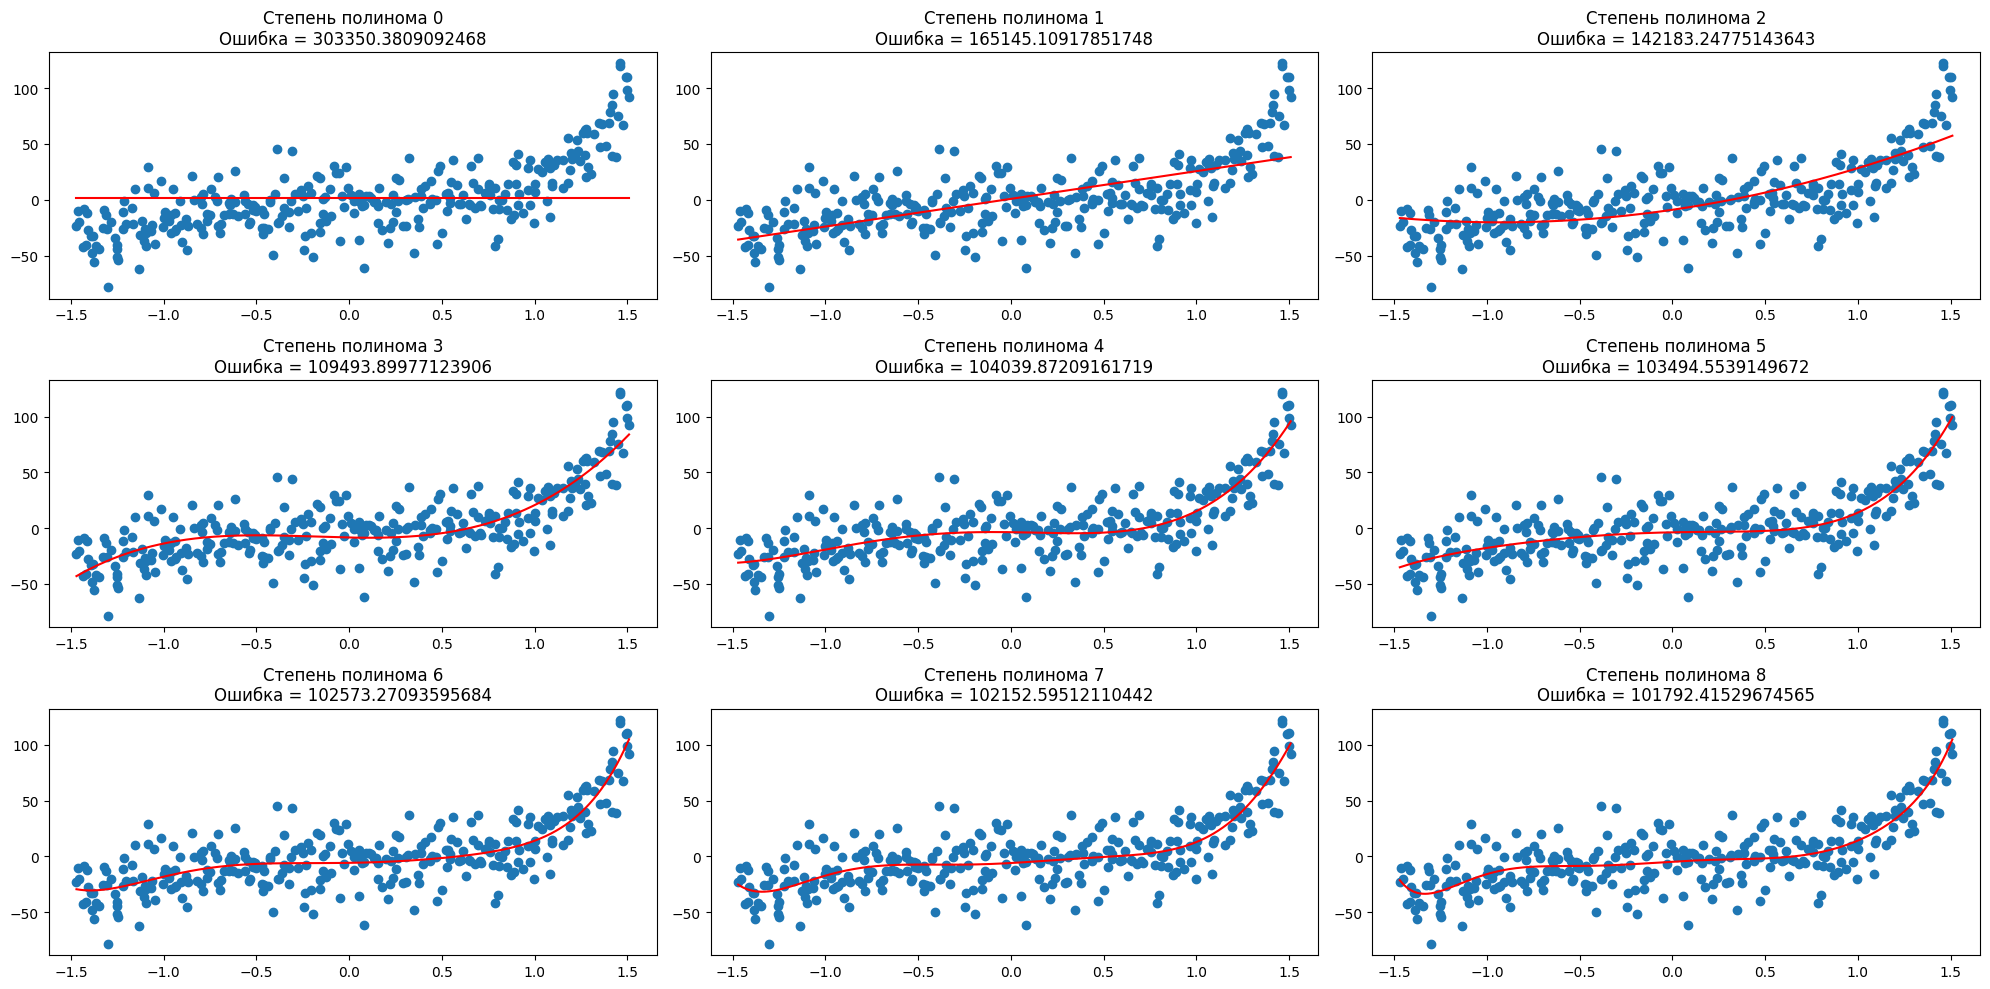
\includegraphics[width=1\textwidth]{img/4_1.png}
	    \caption{Работа полиномиальной регрессии в зависимости от выбранной степени многочлена}
	\end{figure}
	
	\begin{lstlisting}[language=Python, caption=Реализация полиномиальных регрессий с регуляризациями]
			
			def elastic_regression(p, ps, alpha=0.5, lda=1):
			    def rmsprop_loss_f(x, bs, lr, beta, lim=500, eps_mode=False):
			        def loss_diff(x, i):
			            return 2 / len(ps) * sum((sum(ps[k][0] ** j * x[j] for j in range(p + 1)) - ps[k][1]) * ps[k][0] ** i for k in range(len(ps))) + lda * (alpha + (1 - alpha) * x[i])
			
			        def grad(x):
			            indexes = rand_indexes(p + 1, bs)
			            g = np.array([0.0] * (p + 1))
			            for i in indexes:
			                g[i] += loss_diff(x, i)
			            return g
			
			        ee = 1e-6
			        n = len(x)
			        points = []
			        points.append(x)
			        s = 0
			        if eps_mode:
			            while True:
			                g = grad(x)
			                s = s * beta + (1 - beta) * np.dot(g, g)
			                delta = - lr * g / np.sqrt(s + ee)
			                x = x + delta
			
			                points.append(x)
			
			                if len(points) > lim:
			                    return np.array(points)
			        else:
			            for _ in range(lim):
			                g = grad(x)
			                s = s * beta + (1 - beta) * np.dot(g, g)
			                delta = - lr * g / np.sqrt(s + ee)
			                x = x + delta
			                points.append(x)
			
			        return np.array(points)
			
			    x = np.array([0.0] * (p + 1))
			    return rmsprop_loss_f(x, 1, 1.0, 0.99, lim=500)[-1], None
			
			
			def l1_regression(p, points, lda=1):
			    return elastic_regression(p, points, 0, lda)
			
			
			def l2_regression(p, points, lda=1):
			    return elastic_regression(p, points, 1, lda)
			
		\end{lstlisting}
		
		\begin{figure}[ht]
				\centering
				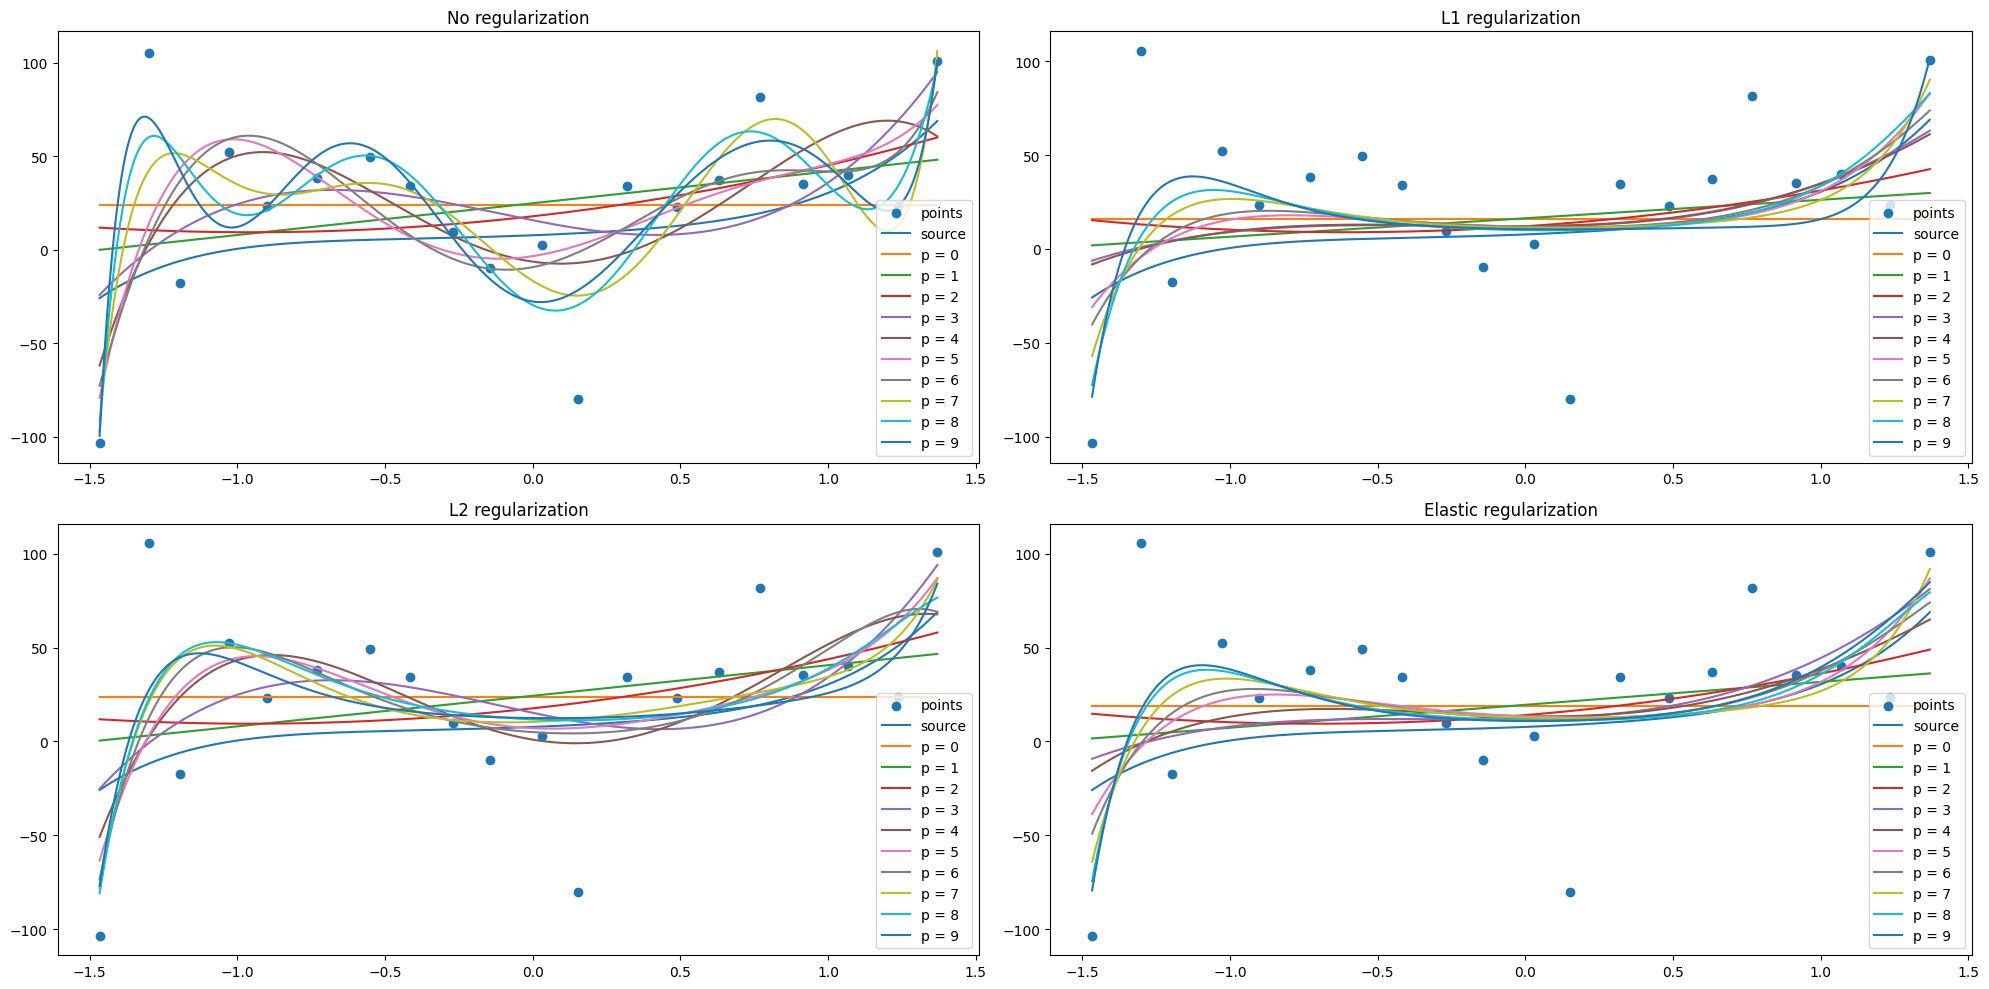
\includegraphics[width=1\textwidth]{img/4_2.png}
			    \caption{Работа полиномиальной регрессии c различными регуляризациями}
			\end{figure}
			
			\newpage
		\subsection{Выводы}
			\begin{itemize}
				\item На иллюстрациях видно, что различные методы регуляризации успешно справляются с тем, чтобы избежать переобучения.
				\item L1 - регуляризация дает нам более "плоский" график, чем L2, но это может привести к тому, что мы можем упустить какие-то скопления точек.
				\item Elastic-регуляризация по определению является сочетанием L1 и L2, и на ее графике видно, что она находится примерно посередине между графиками тех двух регрессий.
			\end{itemize}
	
\end{document}
